%%%%%%%%%%%%%%%%%%%%%%%%%%%%%%%%%%%%%%%%%%%%%%%%%%%%%%%%%%%%%%%%%%%%%%
% Overleaf (WriteLaTeX) Example: Molecular Chemistry Presentation
%
% Source: http://www.overleaf.com
%
% In these slides we show how Overleaf can be used with standard
% chemistry packages to easily create professional presentations.
%
% Feel free to distribute this example, but please keep the referral
% to overleaf.com
%
%%%%%%%%%%%%%%%%%%%%%%%%%%%%%%%%%%%%%%%%%%%%%%%%%%%%%%%%%%%%%%%%%%%%%%

\documentclass[xcolor={dvipsnames}]{beamer}

\mode<presentation>
{
  \usetheme{Madrid}       % or try default, Darmstadt, Warsaw, ...
  \usecolortheme{default} % or try albatross, beaver, crane, ...
  \usefonttheme{default}    % or try default, structurebold, ...
  \setbeamertemplate{navigation symbols}{}
  \setbeamertemplate{caption}[numbered]
}

\usepackage[english]{babel}
\usepackage[utf8x]{inputenc}
\usepackage{graphicx}
\usepackage{hyperref}
  \hypersetup{colorlinks=true}
  \hypersetup{urlcolor=blue}
  \hypersetup{linkcolor = .}
\usepackage{xcolor}
\usepackage{siunitx}
  \sisetup{separate-uncertainty = true}
\DeclareSIUnit\barn{b}
\usepackage{physics}
\usepackage[font=small,labelfont=bf]{caption}
\usepackage{subcaption}
\usepackage[en-GB]{datetime2}
\usepackage{overpic}
\usepackage{feynmp}
\DeclareGraphicsRule{*}{mps}{*}{}
\usepackage{scalerel}
\newcommand{\mylbrace}[2]{\vspace{#2pt}\hspace{6pt}\scaleleftright[\dimexpr5pt+#1\dimexpr0.06pt]{\lbrace}{\rule[\dimexpr2pt-#1\dimexpr0.5pt]{-4pt}{#1pt}}{.}}
\newcommand{\myrbrace}[2]{\vspace{#2pt}\scaleleftright[\dimexpr5pt+#1\dimexpr0.06pt]{.}{\rule[\dimexpr2pt-#1\dimexpr0.5pt]{-4pt}{#1pt}}{\rbrace}\hspace{6pt}}

% Trim in percent
\usepackage{adjustbox}

% No "Figure" prefix
\setbeamertemplate{caption}{\raggedright\insertcaption\par}

% Nice decay amplitude diagrams
\usepackage{amsmath,amssymb,tikz-cd}

% Strike out text
\usepackage[normalem]{ulem}

% For figures with text overlay
\usepackage{overpic}

% Arrows
\usepackage{tikz}
\newcommand{\tikzmark}[1]{\tikz[remember picture] \node[coordinate] (#1) {#1};}

% Colourbox with line breaks
\newcommand{\cbox}[2][lime!20]{%
  \colorbox{#1}{\parbox{\dimexpr\linewidth-2\fboxsep}{\strut #2\strut}}%
}

% Vector arrows
\usepackage[pdftex]{pict2e}

% Checkmark symbol
\def\checkmark{\tikz\fill[scale=0.4](0,.35) -- (.25,0) -- (1,.7) -- (.25,.15) -- cycle;}

% Copy code
\usepackage{listings}
\lstset{
  basicstyle=\ttfamily\tiny,
  breaklines=true
}

% Definitions from Fabian
\usepackage{xspace}
\usepackage{booktabs}
\def\pip    {{\ensuremath{\pi^+}}\xspace}
\def\pim    {{\ensuremath{\pi^-}}\xspace}
\def\Kp     {{\ensuremath{K^+}}\xspace}
\def\Km     {{\ensuremath{K^-}}\xspace}
\def\Dz     {{\ensuremath{D^0}}\xspace}
\def\DKpi   {\ensuremath{\Dz \rightarrow \Km \pip}\xspace}     
\def\DKpipipi   {\ensuremath{\Dz \rightarrow \Km \pip \pip \pim}\xspace} 

% Here's where the presentation starts, with the info for the title slide
\title[RTA WP4 meeting]{Update on 2025 and 2026 tracking efficiencies}

\author[Martin Tat]{Rowina Caspary$^1$, Michel De Cian$^2$, Fabian Glaser$^1$, Stephanie Hansmann-Menzemer$^1$, Peilian Li$^3$, Maurice Morgenthaler$^1$, \\ \textbf{Martin Tat}$^1$}
\institute[Heidelberg]{Heidelberg University$^1$, University of Manchester$^2$, UCAS$^3$}
\date{4th June 2026}

\titlegraphic{
\includegraphics[height = 1.2cm]{../lhcb.jpg}\hspace{1.0cm}~%
              
\includegraphics[height = 1.2cm]{../FSP_logo.png}
              
\includegraphics[height = 1.2cm]{../ManchesterLogo.jpg}~%
              
\includegraphics[height = 1.2cm]{../UCAS_logo.png}~%
              
\includegraphics[height = 1.2cm]{../HeidelbergLogo.pdf}}

\begin{document}

\begin{frame}
  \titlepage
\end{frame}

% These three lines create an automatically generated table of contents.
%\begin{frame}{Outline}
%  \tableofcontents
%\end{frame}

\begin{frame}{Tag-and-probe method}
  \vspace{0.0cm}
  \begin{figure}[htb]
    \centering
    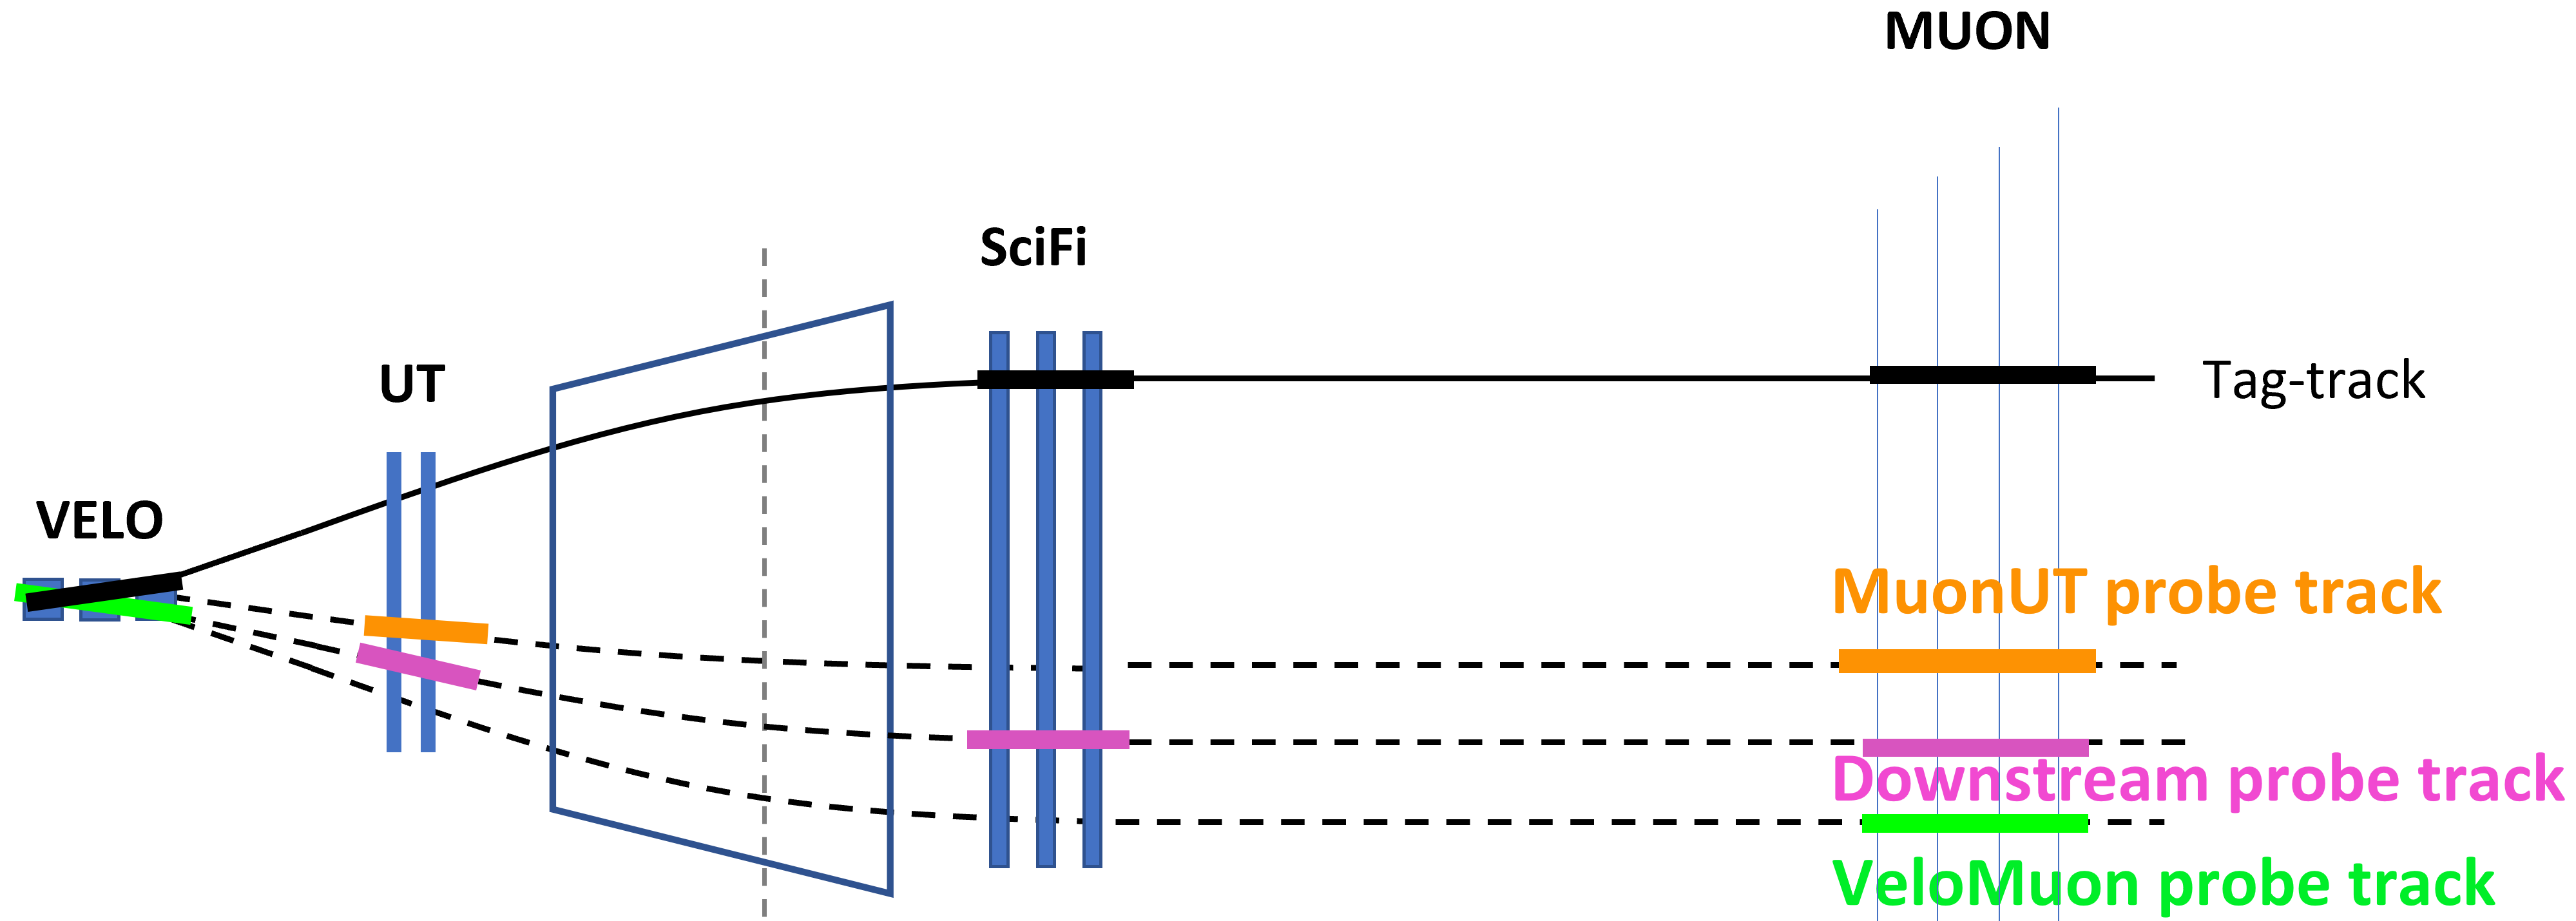
\includegraphics[width=0.75\textwidth]{Plots/Tag_and_probe_method.png}
    \caption*{\tiny Figure by Rowina}
  \end{figure}
  \vspace{-0.1cm}
  \begin{itemize}
    \item{Tag-and-probe method with $J/\psi\to\mu^+\mu^-$}
    \item{Fully reconstruct one muon...}
    \item{... and partially reconstruct the other muon}
    \item{Match hits in specific sub-detector with partially reconstructed track}
  \end{itemize}
  \begin{equation*}
    \epsilon_{\rm track} = \frac{N_{\rm matched}}{N_{\rm matched} + N_{\rm failed}}
  \end{equation*}
\end{frame}

\begin{frame}{Introduction to methods}
  \vspace{0.0cm}
  {\Large Strategy for tracking efficiency determination:}
  \vspace{0.2cm}
  \begin{itemize}
    \setlength\itemsep{0.8em}
    \item{Combine efficiencies of two methods:}
    \begin{itemize}
      \item{VeloMuon: SciFi efficiency}
      \item{Downstream: Velo efficiency}
      \item{Combined: Velo $\times$ SciFi efficiencies}
    \end{itemize}
    \item{Cross check with long track efficiency from the MuonUT method}
    \begin{itemize}
      \item{Main systematic}
    \end{itemize}
  \end{itemize}
\end{frame}

\begin{frame}{Overview of work}
  \vspace{0.0cm}
  {Recent presentations:}
  \vspace{0.2cm}
  \begin{itemize}
    \setlength\itemsep{0.5em}
    \item{\href{https://indico.cern.ch/event/1675248/\#80-trackcalib-for-run-3}{A/S week}}
    \begin{itemize}
      \item[-]{2024 v0 tables available on GitLab \href{https://gitlab.cern.ch/lhcb-rta/tracking-efficiencies-run-3}{here}}
    \end{itemize}
    \item{\href{https://indico.cern.ch/event/1577595/\#4-update-track-reconstruction}{RTA WP4 talk on muon tracking efficiencies}}
    \item{\href{https://indico.cern.ch/event/1577599/\#3-hadronic-tracking-uncertaint}{RTA WP4 talk on hadronic corrections}}
  \end{itemize}
  \vspace{0.5cm}
  {Tracking efficiencies are determined using TrackCalib2}
  \vspace{0.2cm}
  \begin{itemize}
    \setlength\itemsep{0.5em}
    \item{GitLab repository \href{https://gitlab.cern.ch/lhcb-rta/trackcalib2}{here}}
    \item{Mass fit done on tuples from AP to extract efficiencies}
    \item{Note: Analysts should \underline{not} have to run TrackCalib2 themselves, unless the released numbers are not suitable (need different binning, etc)}
  \end{itemize}
\end{frame}

\begin{frame}{Datasets considered}
  \vspace{0.0cm}
  {\large Datasets considered:}
  \vspace{0.2cm}
  \begin{itemize}
    \setlength\itemsep{1.0em}
    \item{2024}
    \begin{itemize}
      \item[-]{v0 results for blocks 2, 1, 5, 6, 7, 8, $pp$ ref available}
      \item[-]{Currently waiting for large MC production (16M per block) to finish}
      \item[-]{Blocks 4 and 3 don't have MC yet}
    \end{itemize}
    \item{2025}
    \begin{itemize}
      \item[-]{Today: Analysis of pre-TS data}
      \item[-]{Post-TS MC in production (4M per block)}
      \item[-]{Very small (100k) post-TS MC samples available for initial checks}
    \end{itemize}
    \item{2026}
    \begin{itemize}
      \item[-]{Today: First look at data}
      \item[-]{Realistic MC not available yet}
    \end{itemize}
  \end{itemize}
\end{frame}

\begin{frame}{Example mass fit}
  \vspace{0.0cm}
  {\large Example of fit to extract efficiency (2024 block 5, 1D $\eta$ bin 3)}
  \begin{figure}[htb]
    \centering
    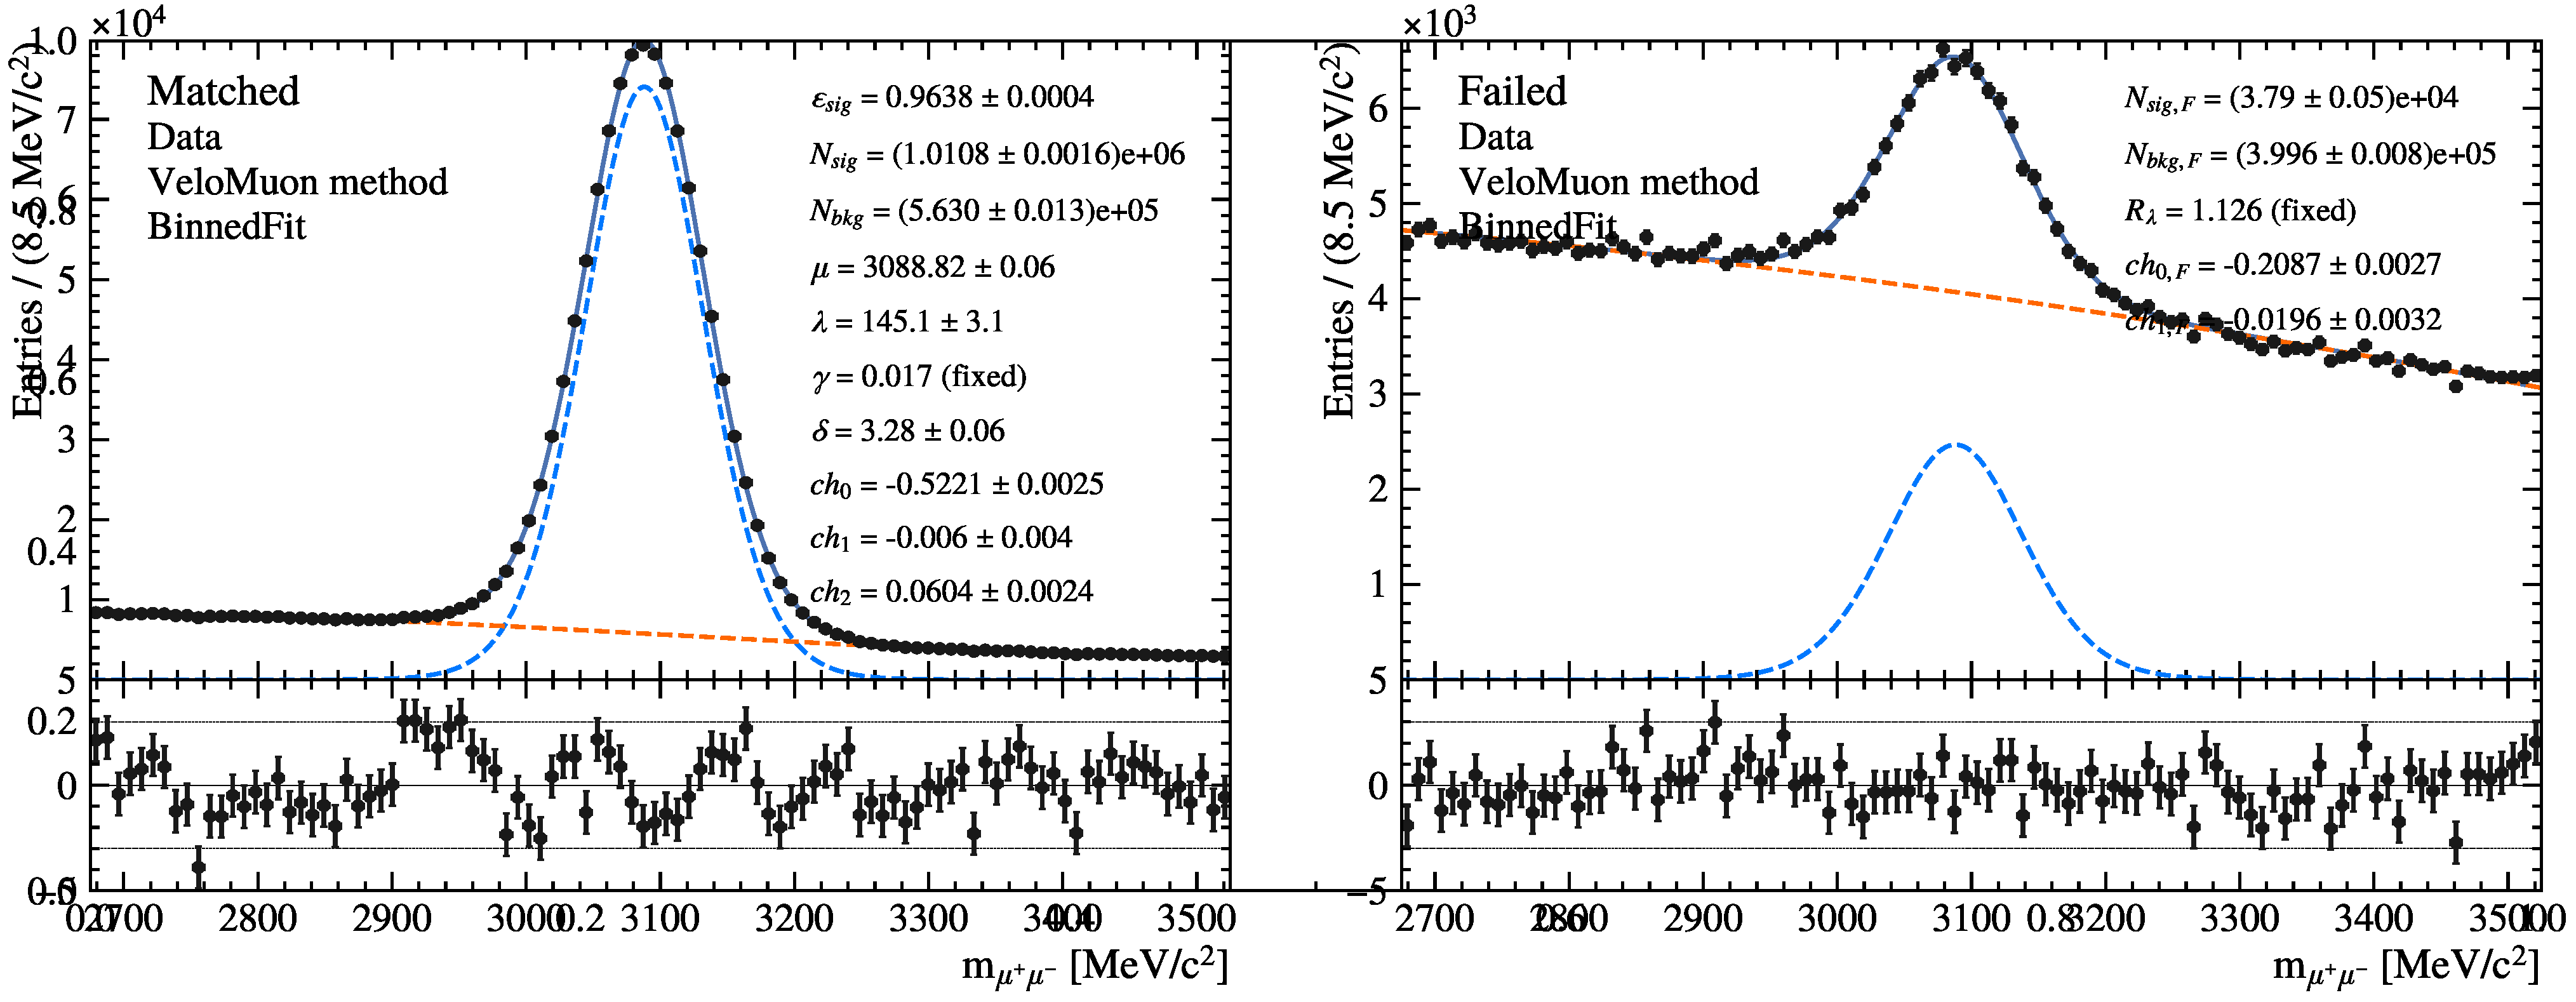
\includegraphics[width=0.85\textwidth]{Plots/Data_VeloMuon_ETA_3_sim.pdf}
  \end{figure}
  \begin{itemize}
    \item{Efficiency is a free parameter in the fit}
    \item{Matched and failed samples simultaneously fitted to ensure correct uncertainties}
  \end{itemize}
\end{frame}

\begin{frame}{2025 block definitions}
  \vspace{0.0cm}
  {\large Define 2025 blocks according to simulation conditions:}
  \vspace{0.2cm}
  \begin{center}
    \begin{table}[htb]
      \begin{center}
        \begin{tabular}{cccccc}
          \hline
          Block & Sprucing campaign & Magnet polarity & MC sample & $\mathcal{L}_{\rm int} ($fb$^{-1})$ \\
          \hline
          $1$   & Sprucing25c1      & MagDown         & W21       & $0.4$ \\
          $2$   & Sprucing25c1      & MagUp           & W22.25    & $1.6$ \\
          $3$   & Sprucing25c2      & MagDown         & W28.36    & $4.3$ \\
          $4$   & Sprucing25c3/4    & MagUp   & W37.43    & $4.1$ \\
          $5$   & Sprucing5c4       & MagDown         & W43.45    & $1.0$ \\
          \hline
        \end{tabular}
      \end{center}
    \end{table}
  \end{center}
\end{frame}

\begin{frame}{2025 data/MC ratios in 1D}
  \vspace{0.0cm}
  {\large 2025 pre-TS data/MC ratios, Block 1}
  \begin{figure}[htb]
    \centering
    \begin{subfigure}{0.5\textwidth}
      \centering
      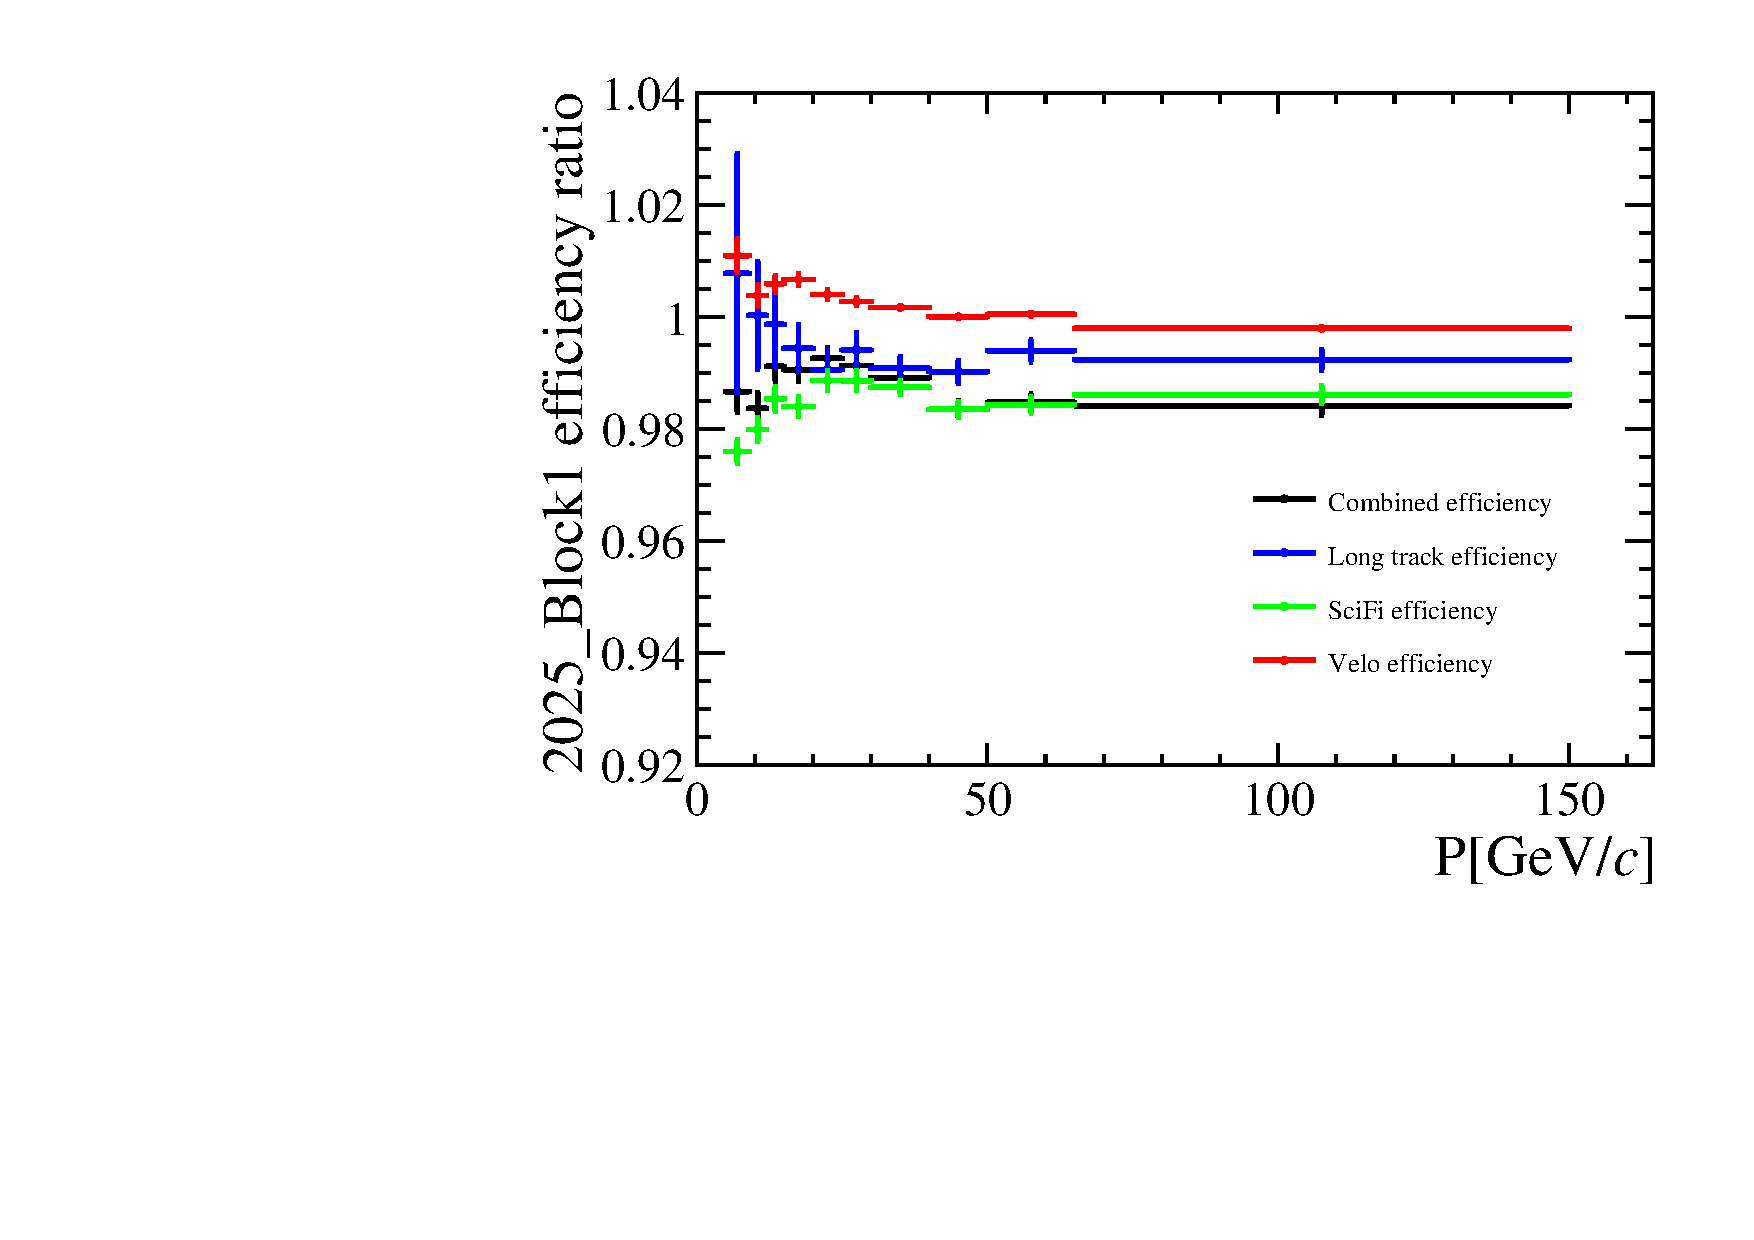
\includegraphics[width=1.0\textwidth]{Plots/trackeff_ratio_P_2025_Block1_workdir_samples.pdf}
    \end{subfigure}%
    \begin{subfigure}{0.5\textwidth}
      \centering
      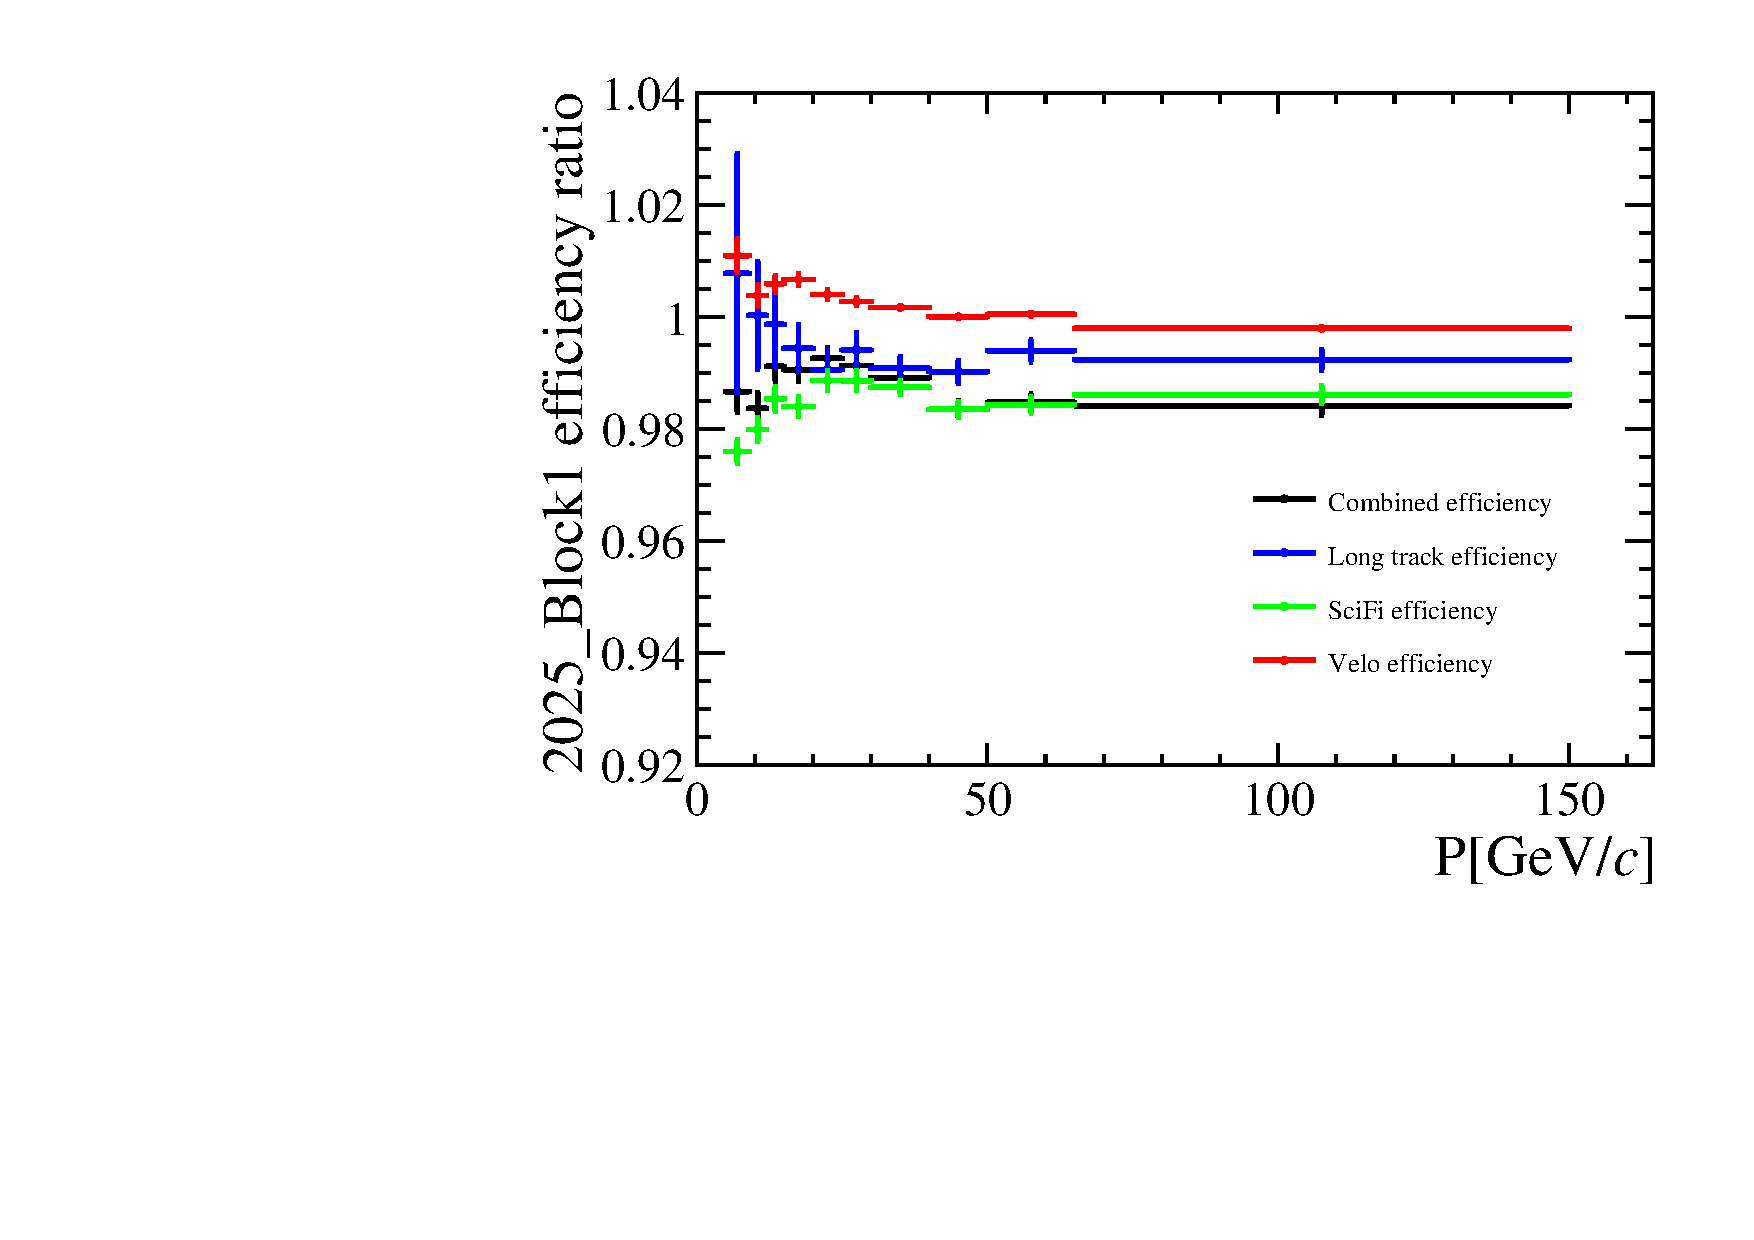
\includegraphics[width=1.0\textwidth]{Plots/trackeff_ratio_P_2025_Block1_workdir_samples.pdf}
    \end{subfigure}
  \end{figure}
  {Note that Velo efficiencies are underestimated for this block!}
\end{frame}

\begin{frame}{2025 data/MC ratios in 1D}
  \vspace{0.0cm}
  {\large 2025 pre-TS data/MC ratios, Block 2}
  \begin{figure}[htb]
    \centering
    \begin{subfigure}{0.5\textwidth}
      \centering
      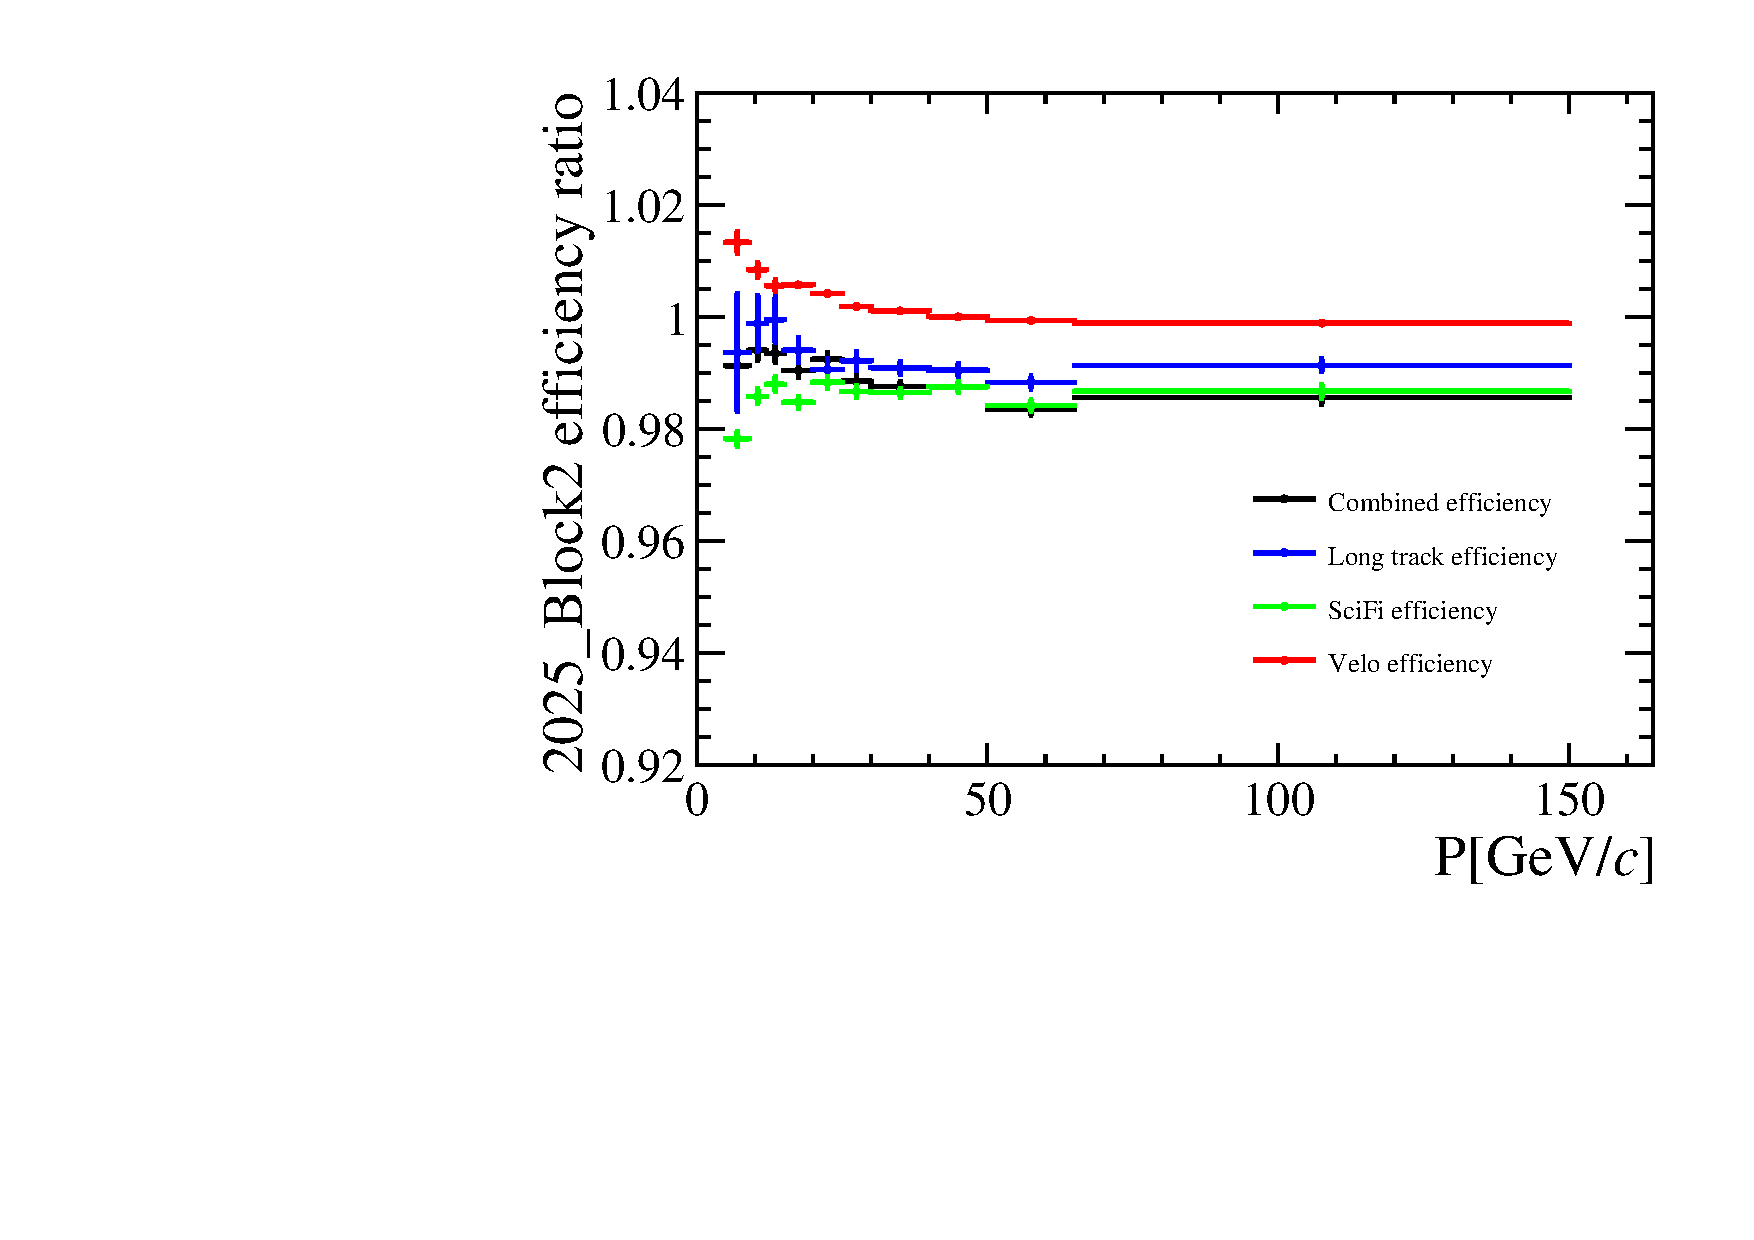
\includegraphics[width=1.0\textwidth]{Plots/trackeff_ratio_P_2025_Block2_workdir_samples.pdf}
    \end{subfigure}%
    \begin{subfigure}{0.5\textwidth}
      \centering
      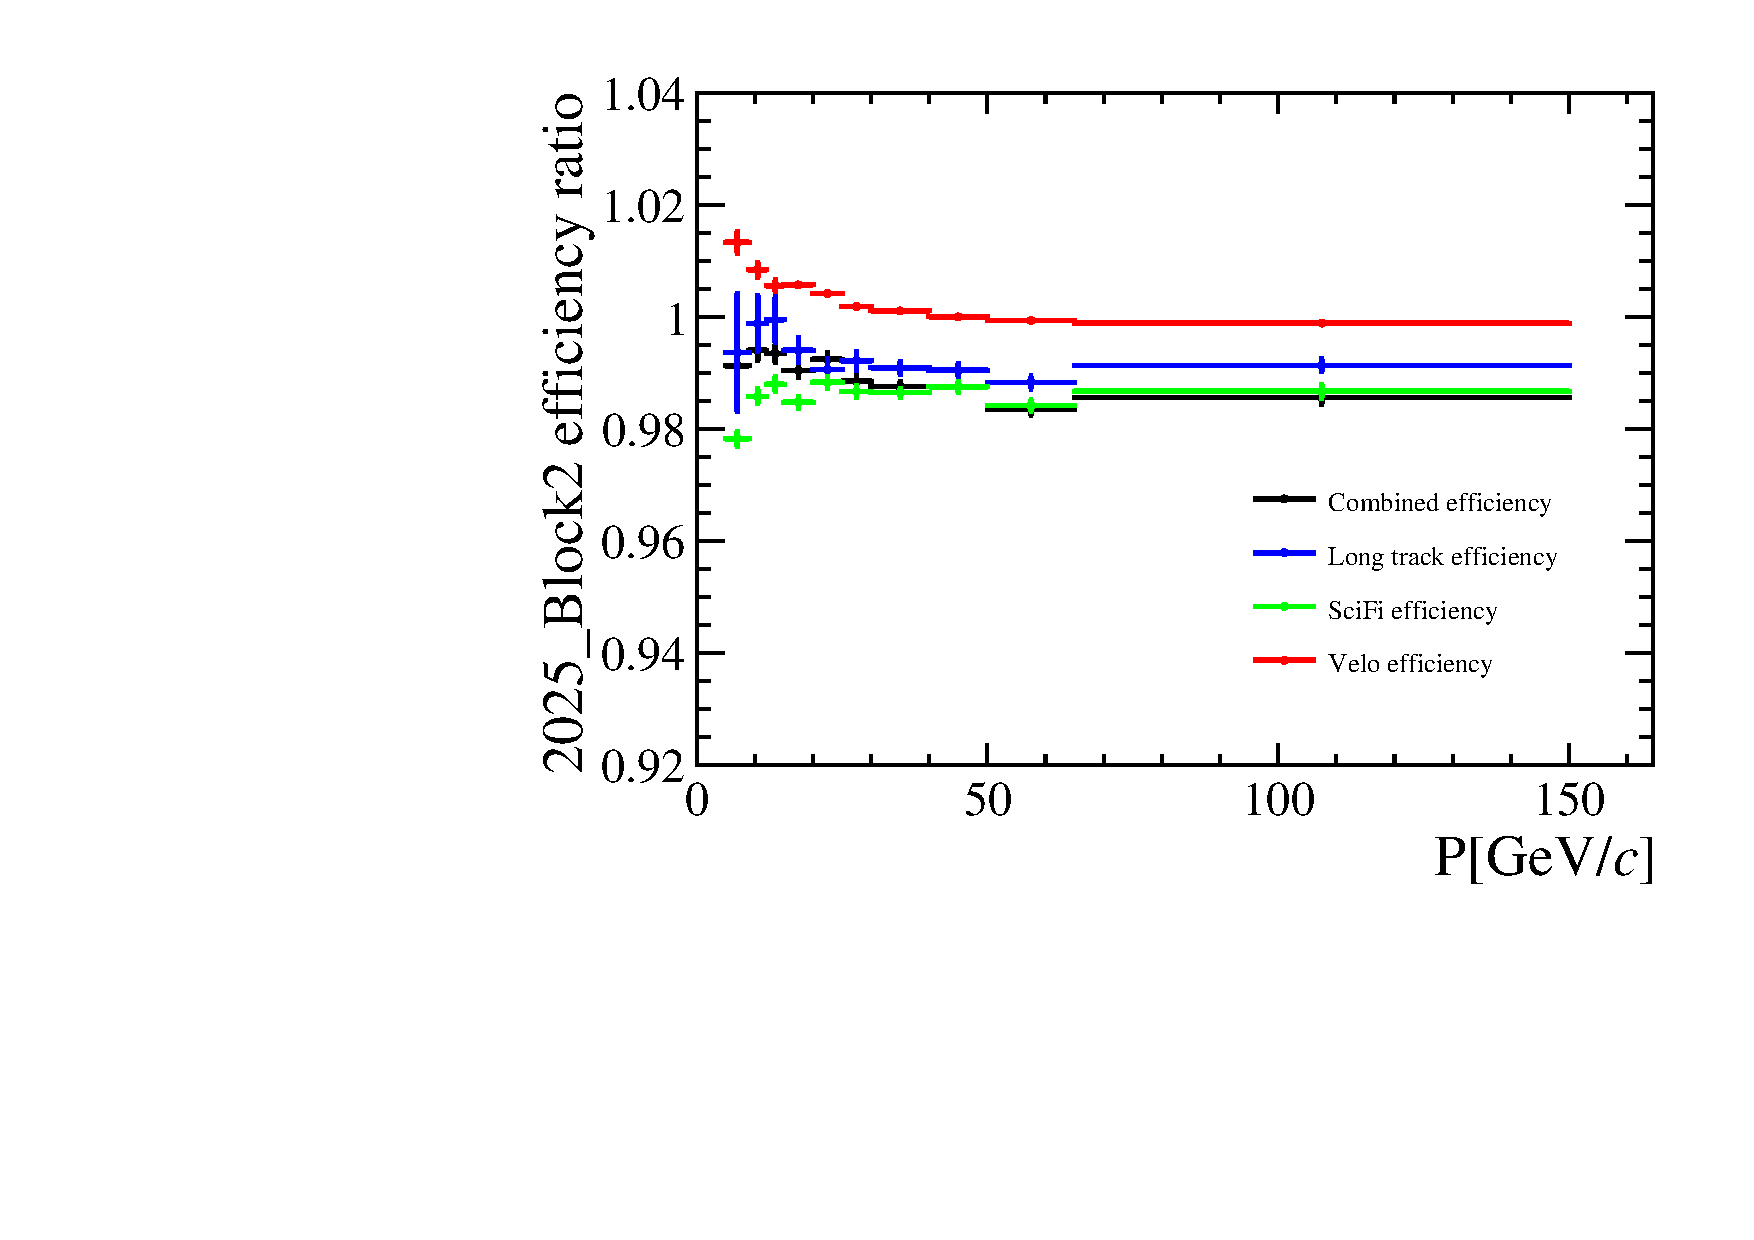
\includegraphics[width=1.0\textwidth]{Plots/trackeff_ratio_P_2025_Block2_workdir_samples.pdf}
    \end{subfigure}
  \end{figure}
  {Note that Velo efficiencies are underestimated for this block!}
\end{frame}

\begin{frame}{2025 data/MC ratios in 1D}
  \vspace{0.0cm}
  {\large 2025 pre-TS data/MC ratios, Block 3}
  \begin{figure}[htb]
    \centering
    \begin{subfigure}{0.5\textwidth}
      \centering
      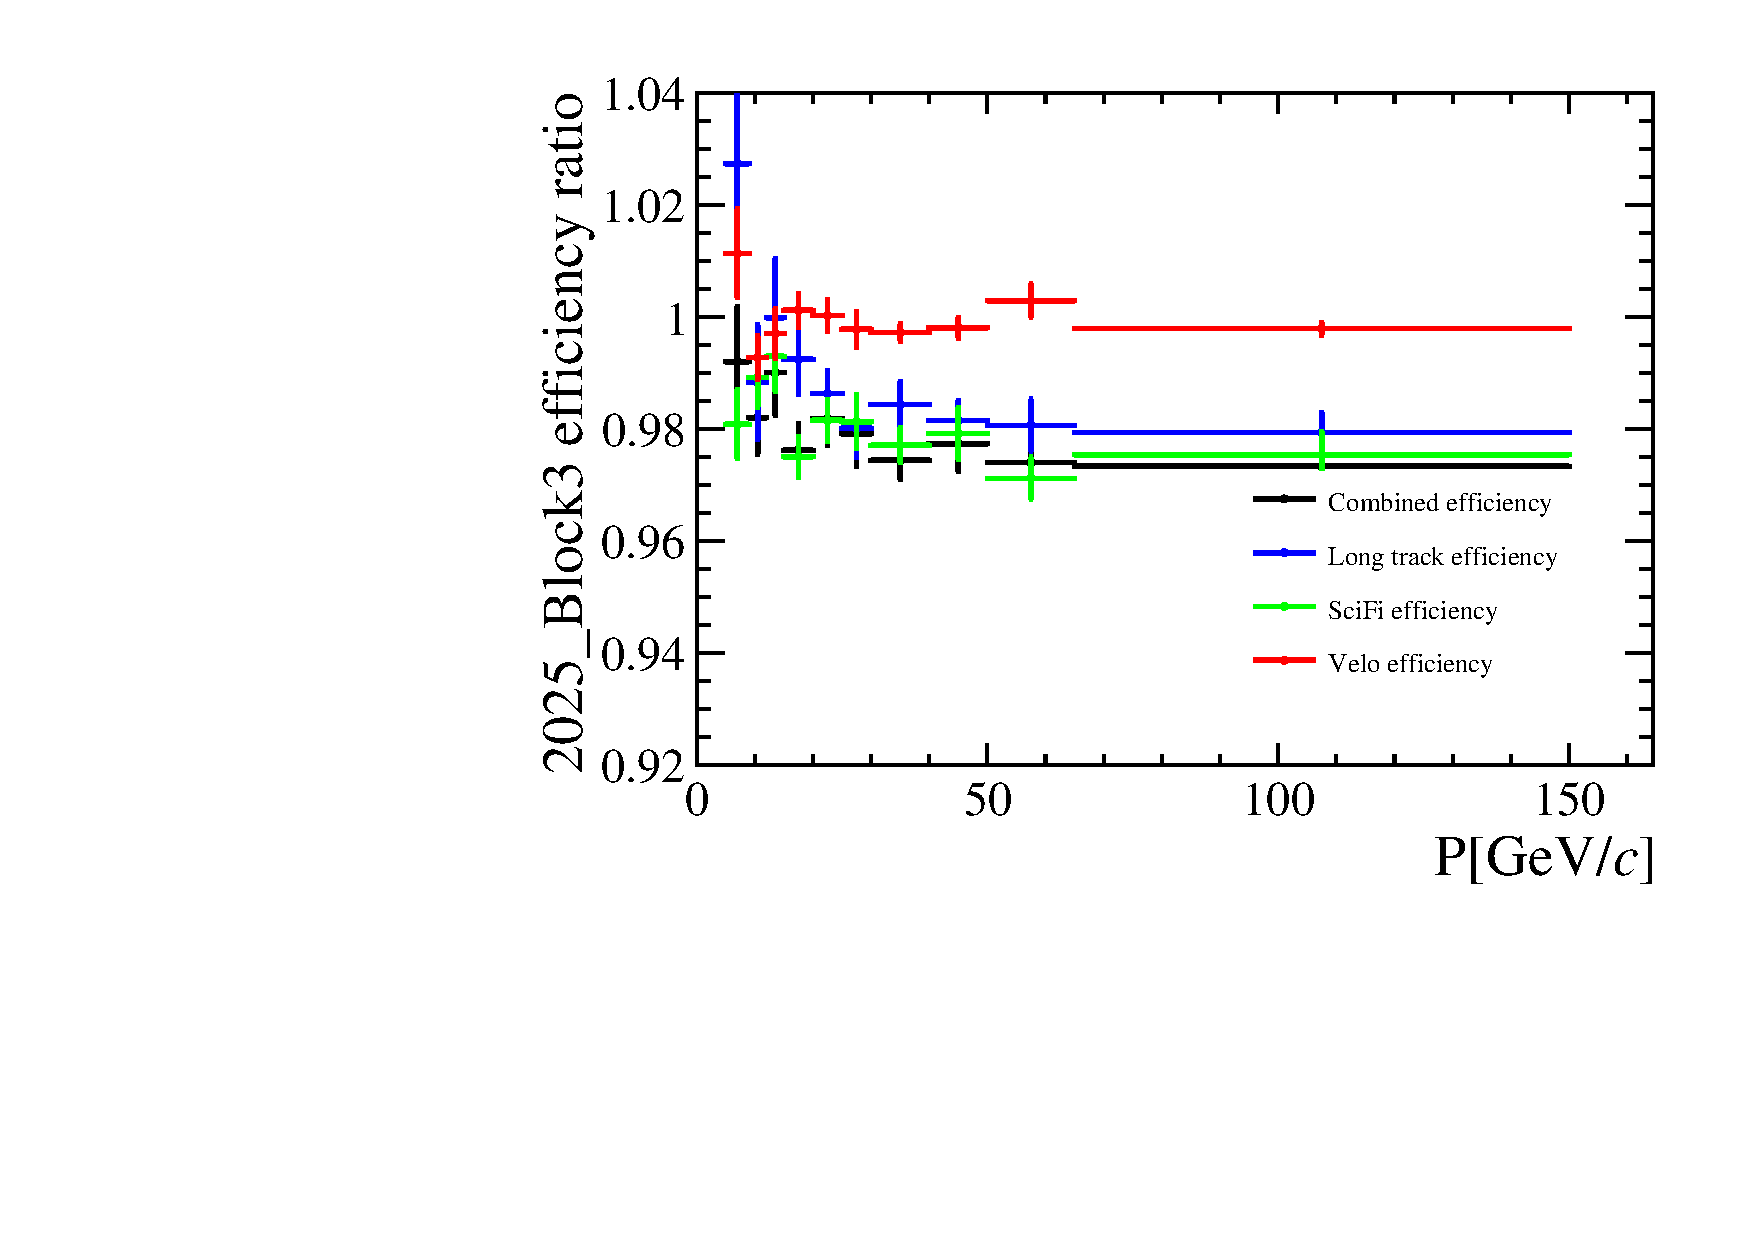
\includegraphics[width=1.0\textwidth]{Plots/trackeff_ratio_P_2025_Block3_workdir_samples.pdf}
    \end{subfigure}%
    \begin{subfigure}{0.5\textwidth}
      \centering
      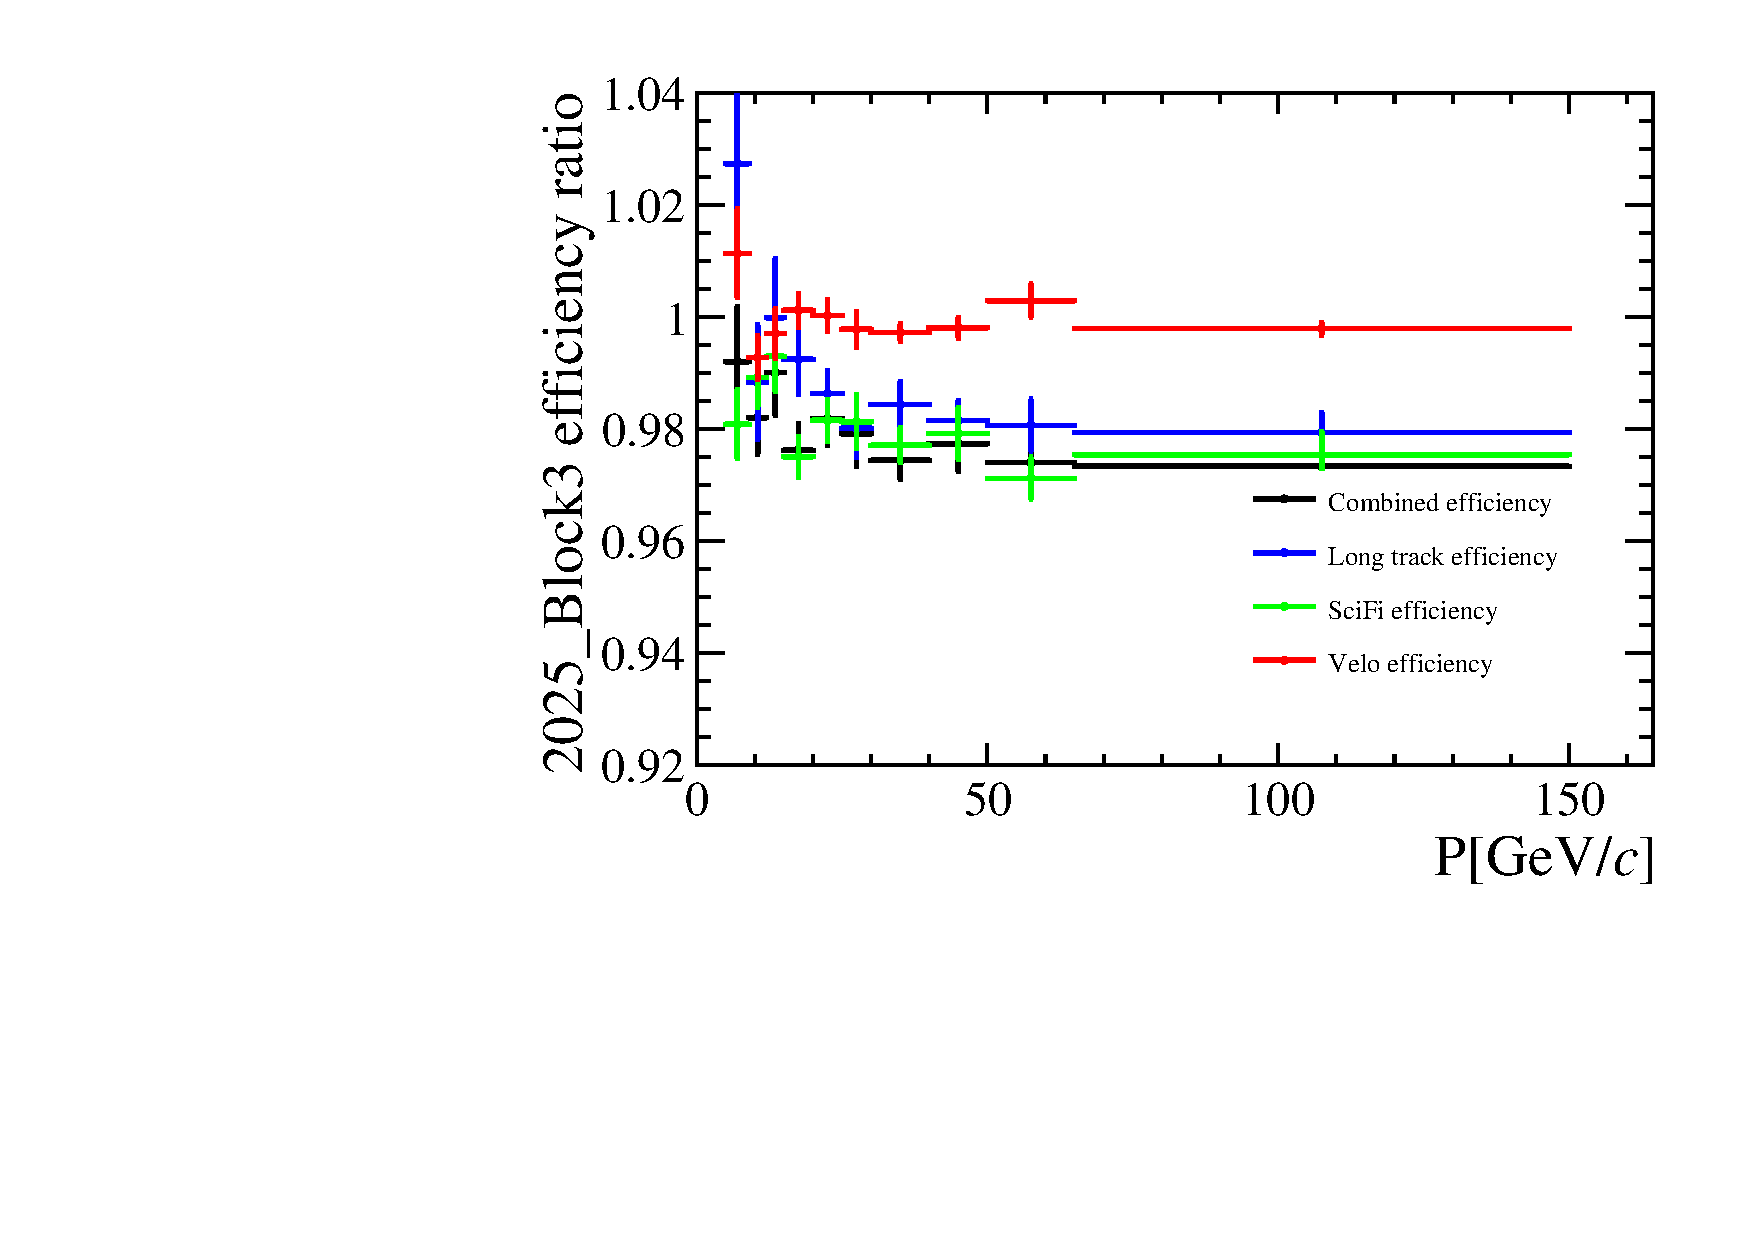
\includegraphics[width=1.0\textwidth]{Plots/trackeff_ratio_P_2025_Block3_workdir_samples.pdf}
    \end{subfigure}
  \end{figure}
  {Better Velo efficiency agreement, but MC statistics very low...}
\end{frame}

\begin{frame}{2025 data/MC ratios in 1D}
  \vspace{0.0cm}
  {\large 2025 pre-TS data/MC ratios, Block 4}
  \begin{figure}[htb]
    \centering
    \begin{subfigure}{0.5\textwidth}
      \centering
      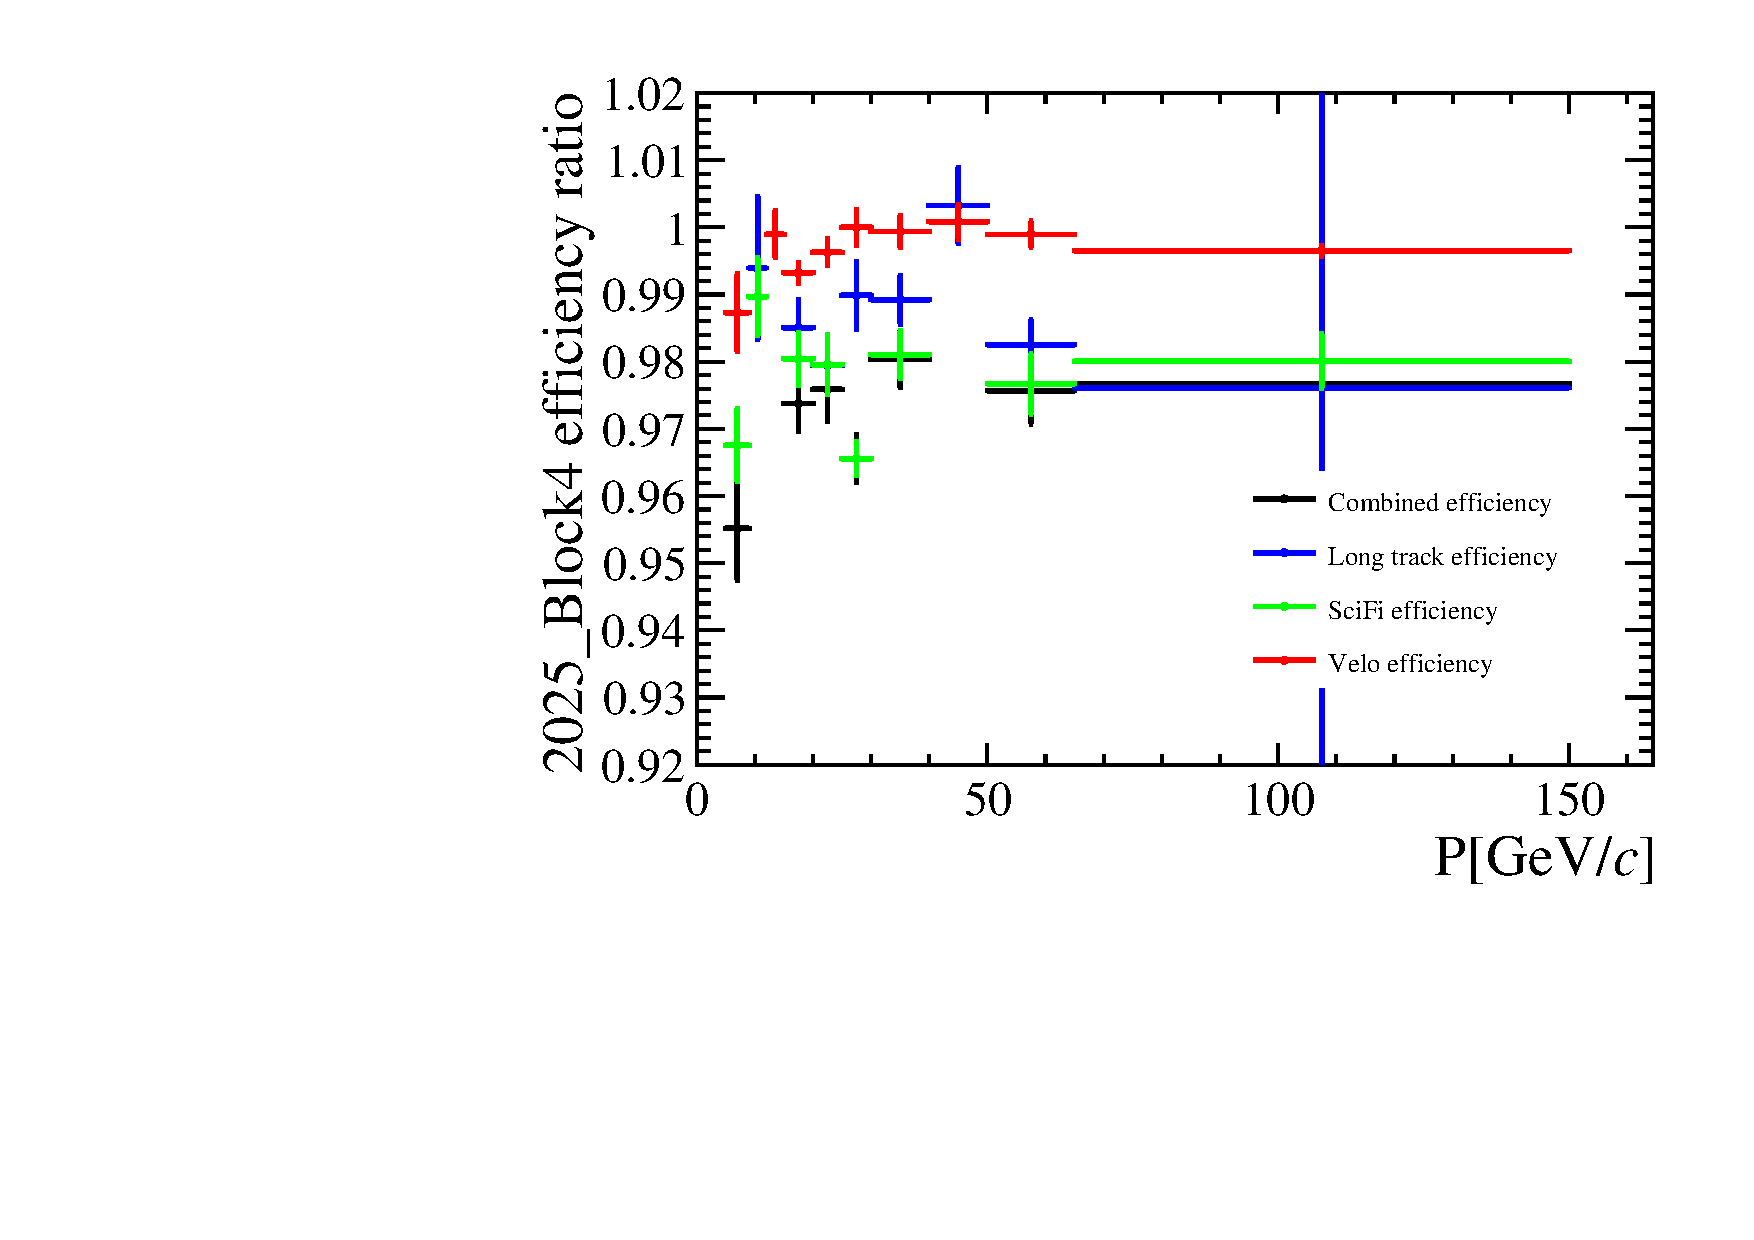
\includegraphics[width=1.0\textwidth]{Plots/trackeff_ratio_P_2025_Block4_workdir_samples.pdf}
    \end{subfigure}%
    \begin{subfigure}{0.5\textwidth}
      \centering
      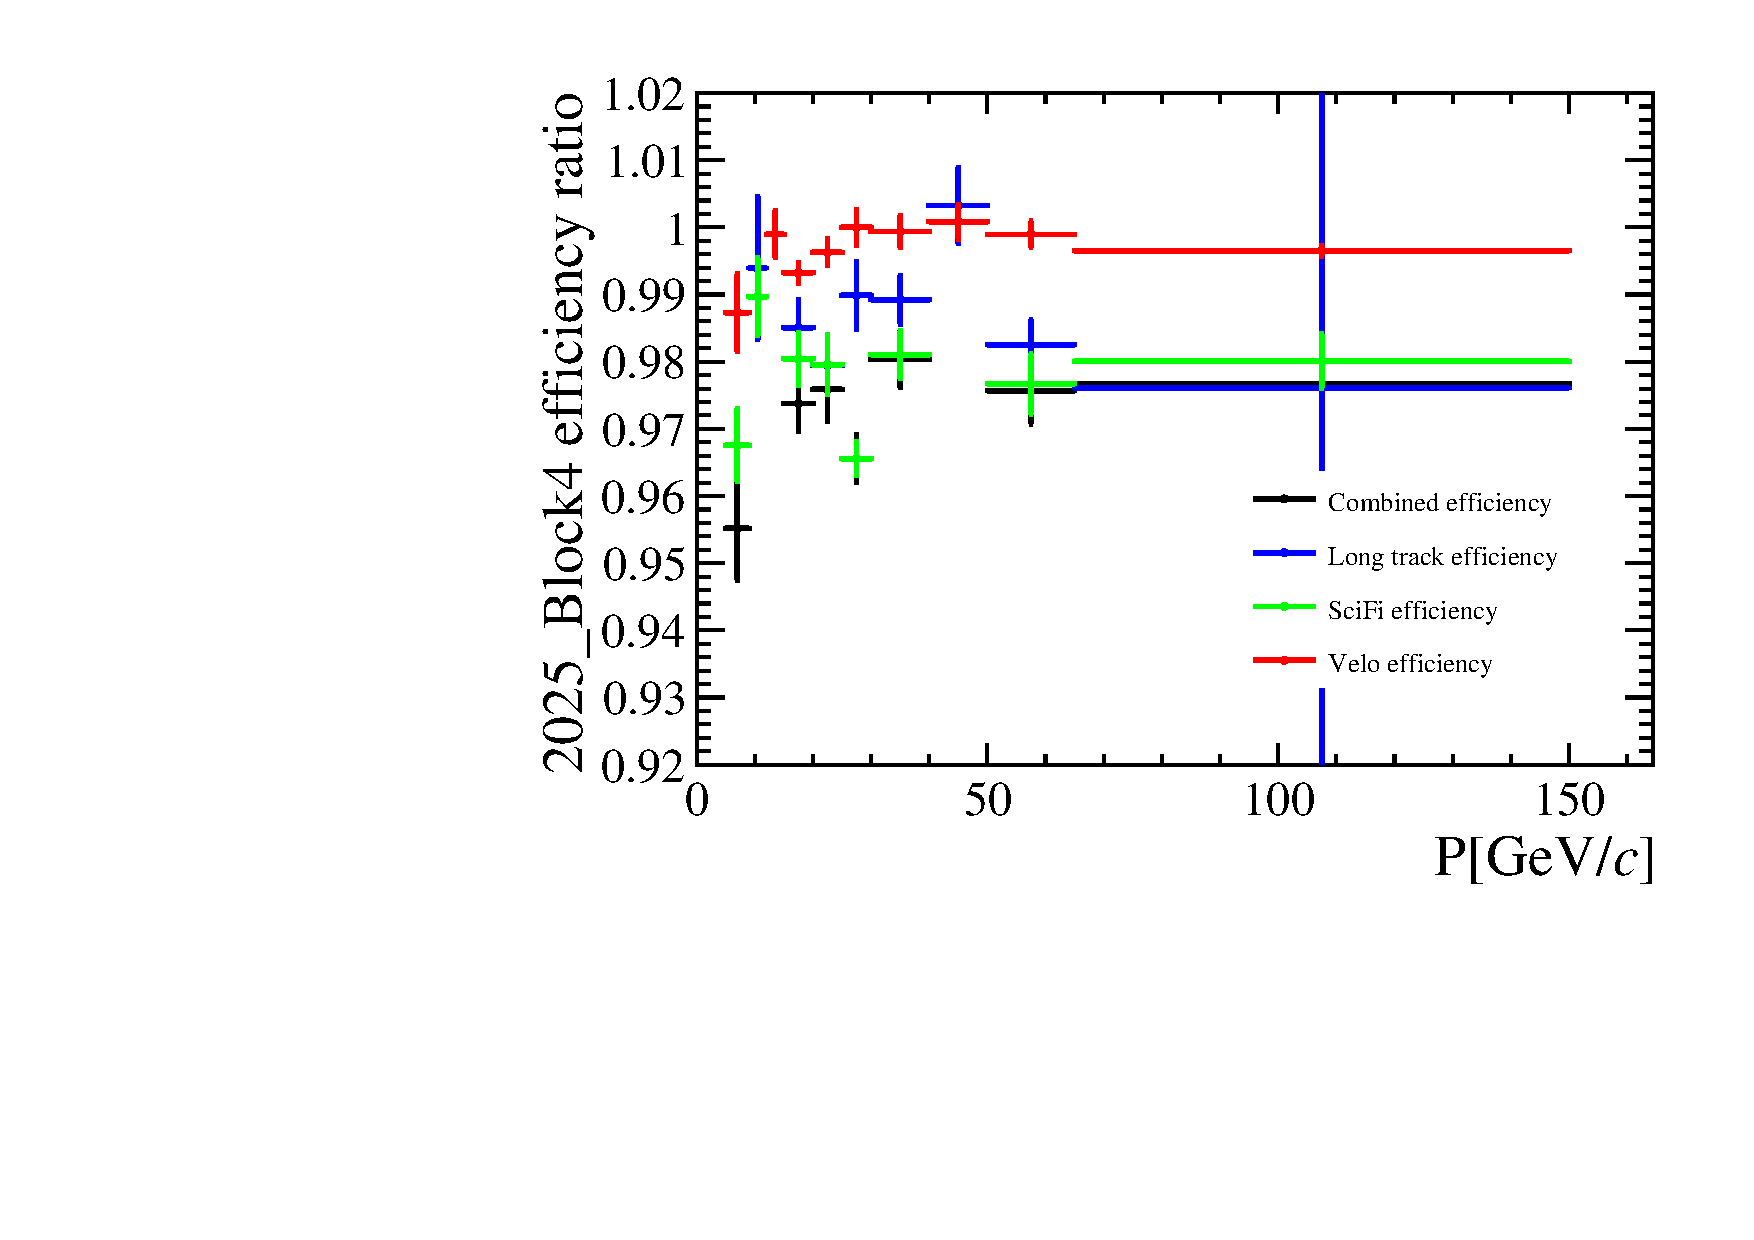
\includegraphics[width=1.0\textwidth]{Plots/trackeff_ratio_P_2025_Block4_workdir_samples.pdf}
    \end{subfigure}
  \end{figure}
  {Better Velo efficiency agreement, but MC statistics very low...}
\end{frame}

\begin{frame}{2025 data/MC ratios in 1D}
  \vspace{0.0cm}
  {\large 2025 pre-TS data/MC ratios, Block 5}
  \begin{figure}[htb]
    \centering
    \begin{subfigure}{0.5\textwidth}
      \centering
      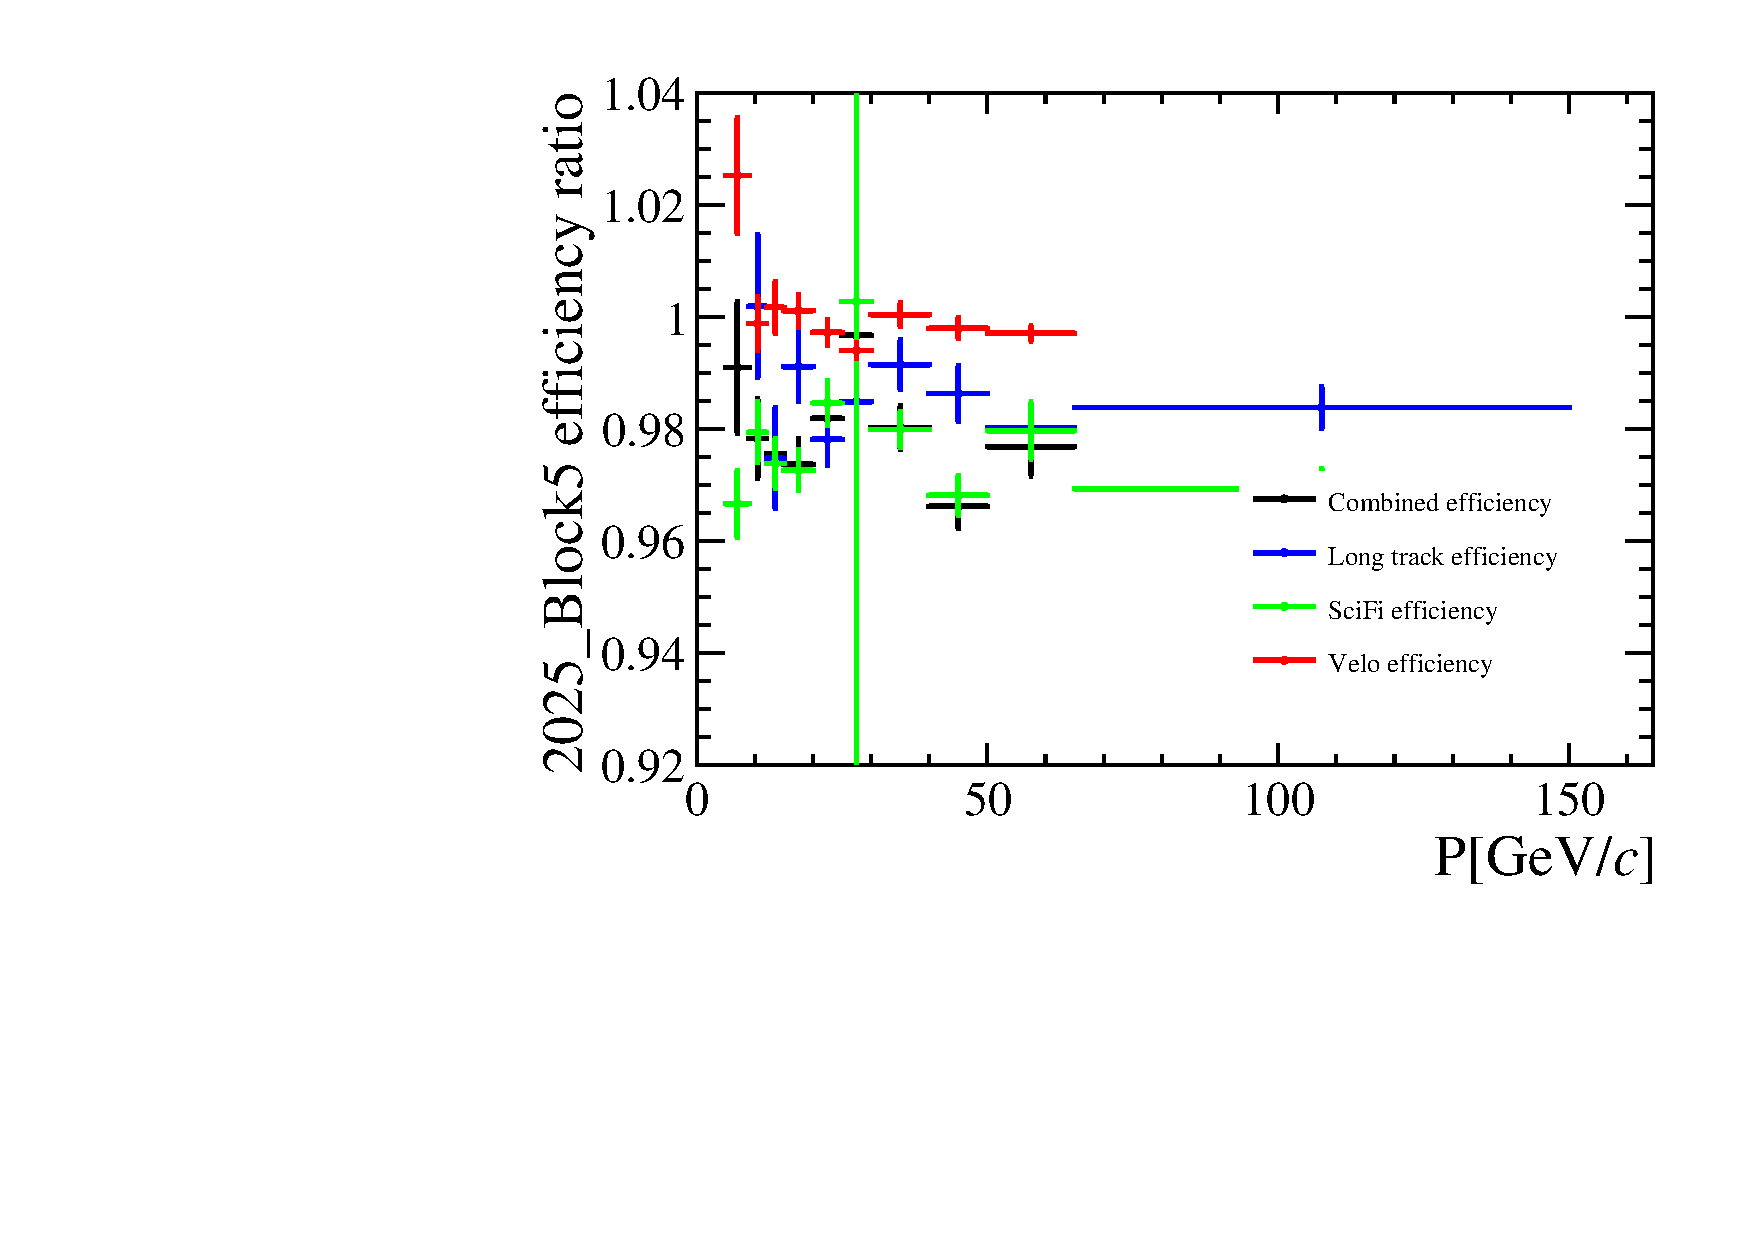
\includegraphics[width=1.0\textwidth]{Plots/trackeff_ratio_P_2025_Block5_workdir_samples.pdf}
    \end{subfigure}%
    \begin{subfigure}{0.5\textwidth}
      \centering
      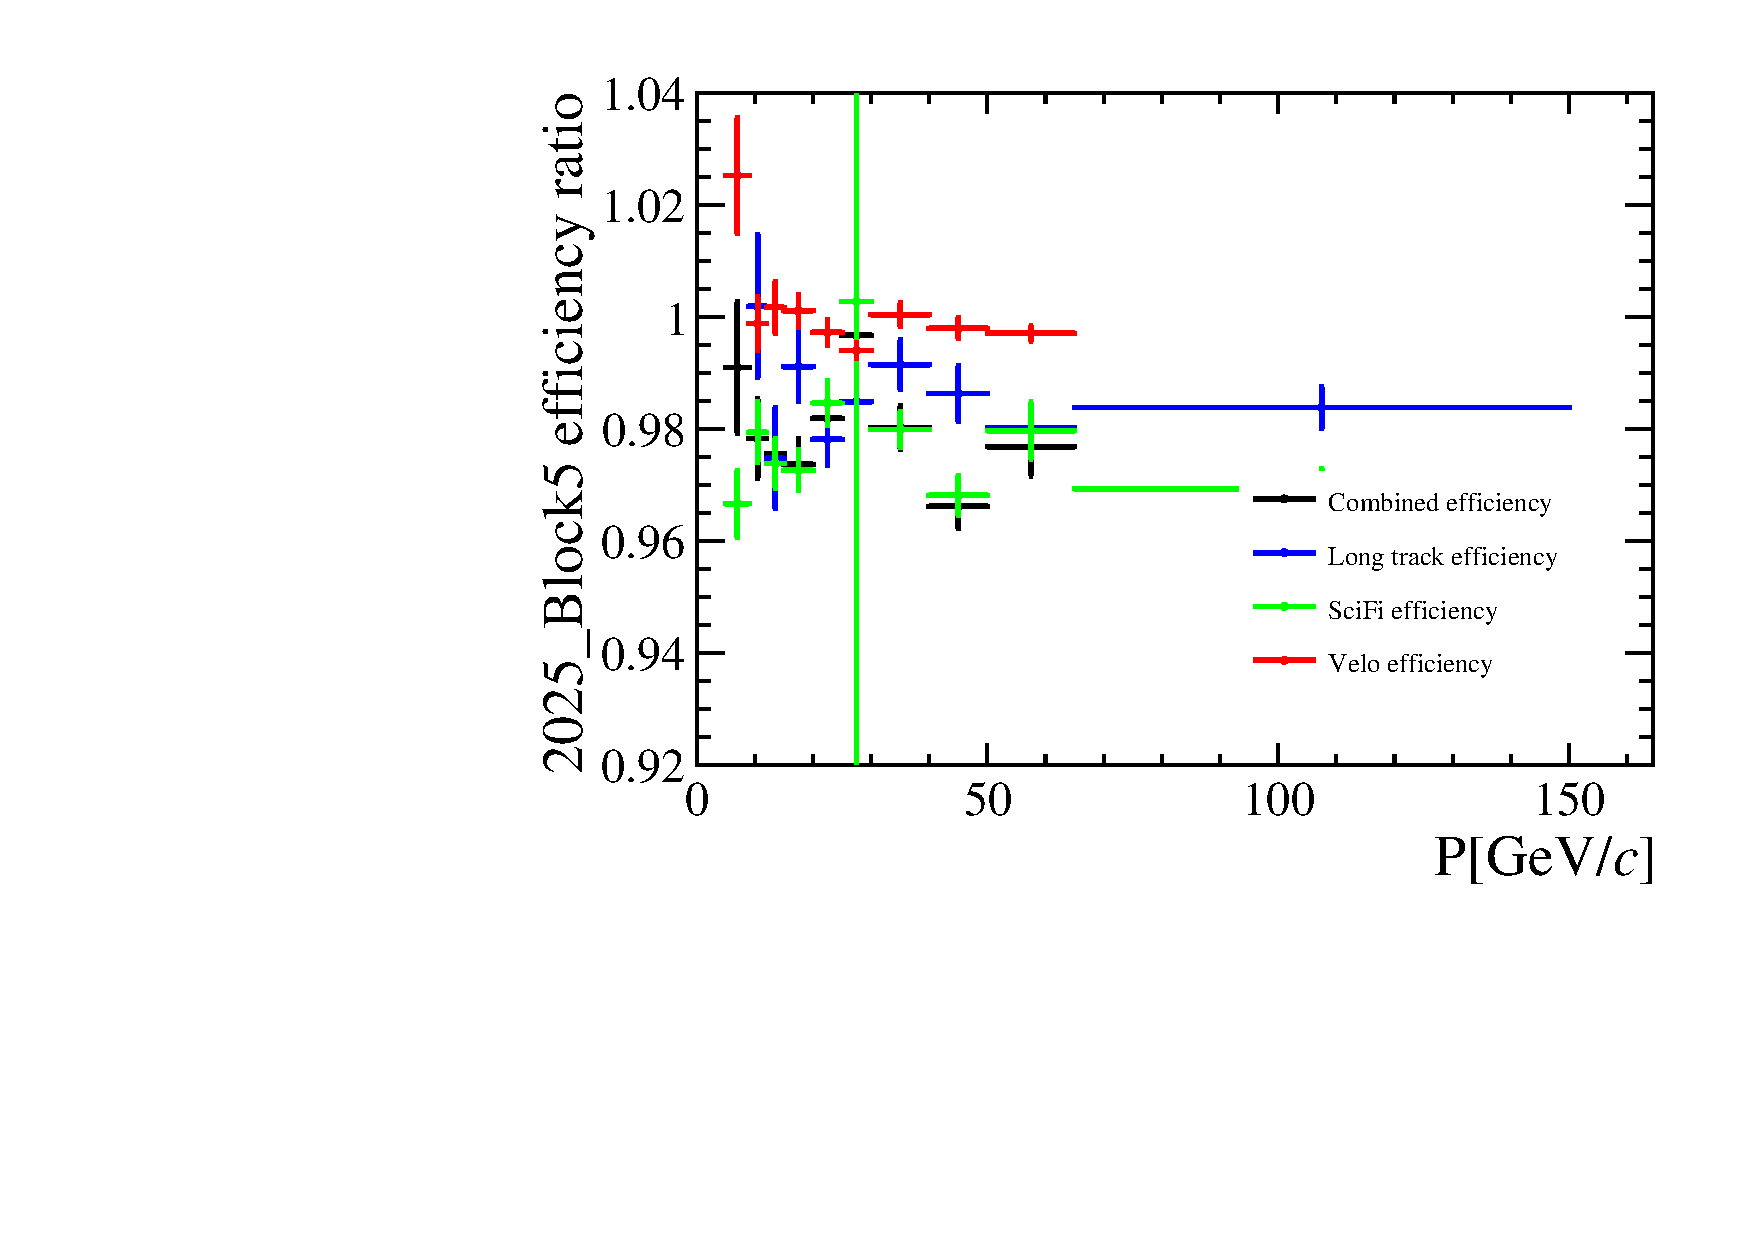
\includegraphics[width=1.0\textwidth]{Plots/trackeff_ratio_P_2025_Block5_workdir_samples.pdf}
    \end{subfigure}
  \end{figure}
  {Better Velo efficiency agreement, but MC statistics very low...}
\end{frame}

\begin{frame}{2025 pre-TS Velo discrepancies}
  \vspace{0.0cm}
  {\large Why are Velo efficiencies underestimated in pre-TS MC?}
  \vspace{0.2cm}
  \begin{itemize}
    \setlength\itemsep{0.8em}
    \item{Velo M23 was (sometimes) working in data, but all four sensors are turned off in MC}
    \item{Two sensors in Velo M21 were turned off}
    \item{Two consecutive modules that are not working properly can significantly impact track efficiency!}
  \end{itemize}
  \begin{figure}[htb]
    \centering
    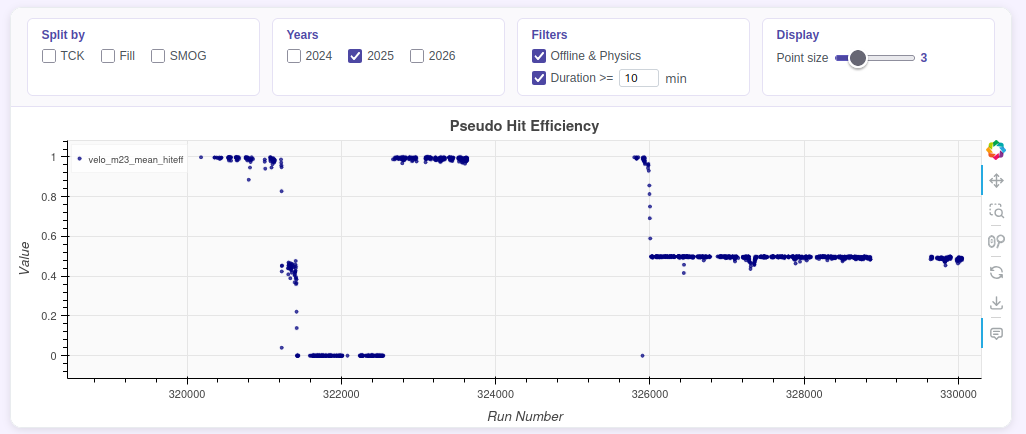
\includegraphics[width=0.65\textwidth]{Plots/Velo_M23_hit_efficiency.png}
    \caption*{M23 hit efficiency during data taking from Intelli RTA}
  \end{figure}
\end{frame}

\begin{frame}{2025 pre-TS Velo discrepancies}
  \vspace{0.0cm}
  {\large Note: Both M21 and M23 are on the A-side, leading to a significant left-right asymmetry}
  \begin{figure}[htb]
    \centering
    \begin{subfigure}{0.5\textwidth}
      \centering
      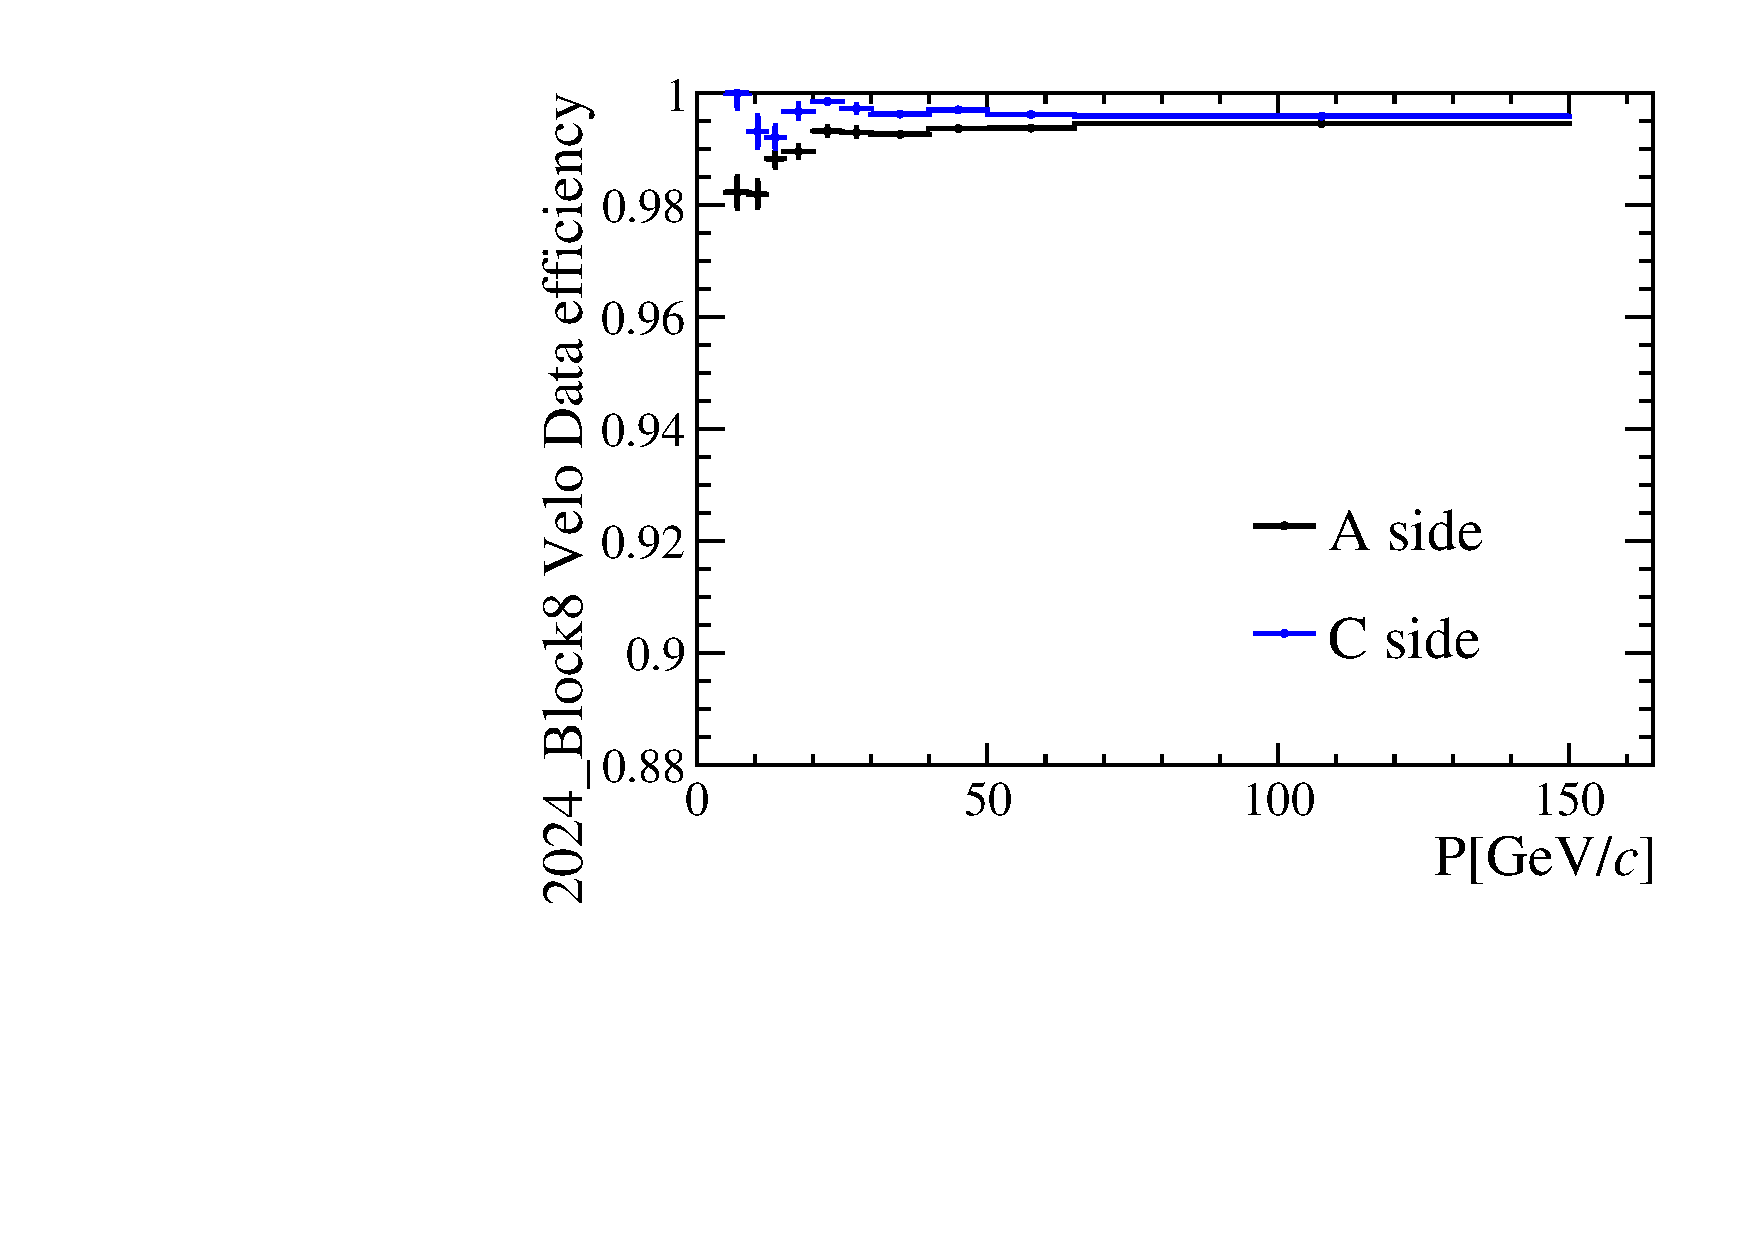
\includegraphics[width=1.0\textwidth]{Plots/trackeff_Data_Downstream_2024_Block8_P_ACside_comparison.pdf}
    \end{subfigure}%
    \begin{subfigure}{0.5\textwidth}
      \centering
      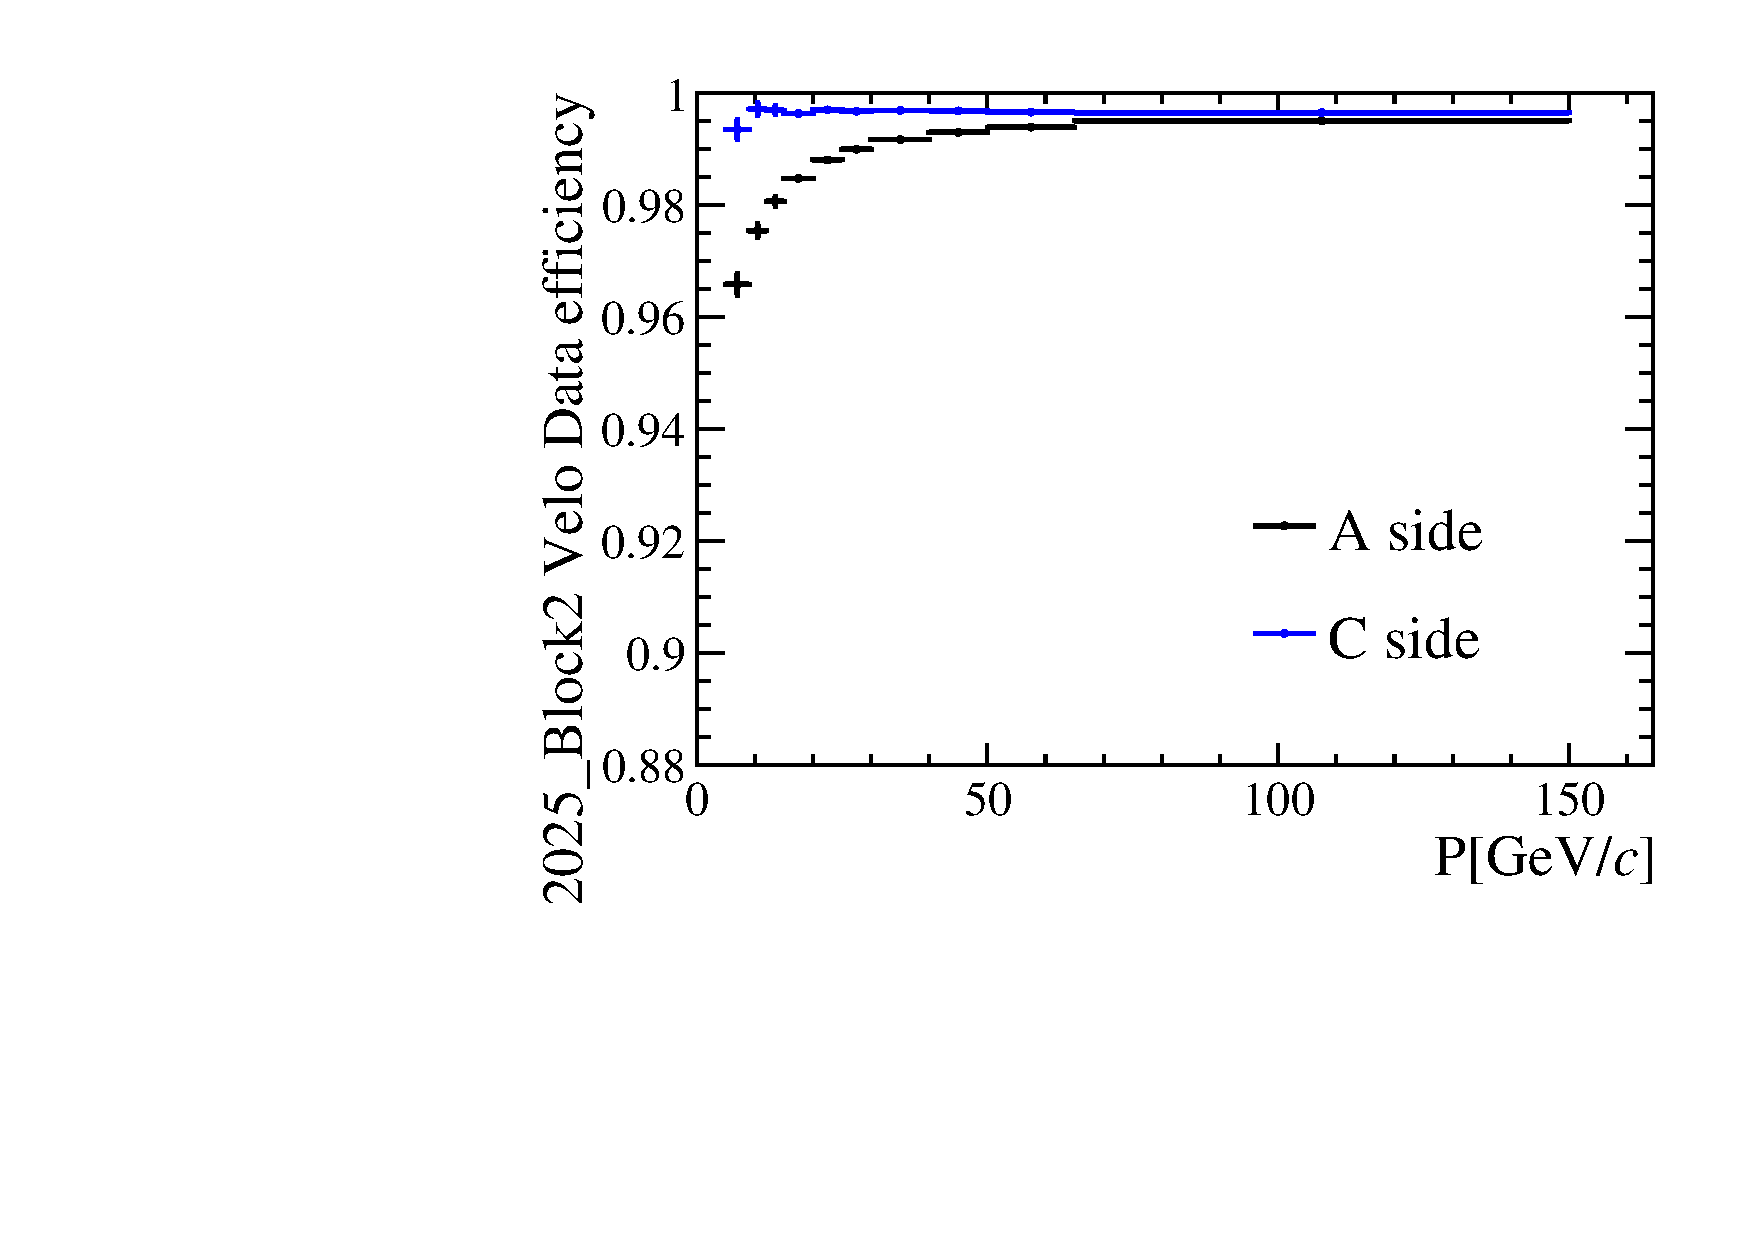
\includegraphics[width=1.0\textwidth]{Plots/trackeff_Data_Downstream_2025_Block2_P_ACside_comparison.pdf}
    \end{subfigure}
  \end{figure}
  {Only M23 was off in 2024, but in 2025 two sensors failed in M21}
\end{frame}

\begin{frame}{2025 pre-TS Velo discrepancies}
  \vspace{0.0cm}
  {\large What are the consequences for tracking efficiencies?}
  \vspace{0.2cm}
  \begin{itemize}
    \setlength\itemsep{0.8em}
    \item{All Sim10g MC samples are affected}
    \item{In principle tracking efficiency corrections should account for this...}
    \item{... but a fix is also in progress: \href{https://gitlab.cern.ch/lhcb-conddb/SIMCOND/-/merge_requests/306}{!306}}
  \end{itemize}
  \vspace{0.5cm}
  {\large What we would like to do about this:}
  \vspace{0.2cm}
  \begin{enumerate}
    \setlength\itemsep{0.8em}
    \item{Request a larger MC production (16M per block) for 2025 pre-TS, with \href{https://gitlab.cern.ch/lhcb-conddb/SIMCOND/-/merge_requests/306}{!306}}
    \item{Change $p$--$\eta$ binning to $p$--$\eta$--$\phi$ with two $\phi$ bins corresponding to left and right ($\abs{\phi} < \pi/2$ and $\abs{\phi} \geq \pi/2$)}
  \end{enumerate}
\end{frame}

\begin{frame}{2D binning}
  \vspace{0.0cm}
  {\large 2D binning in $p$ vs $\eta$ with 72 bins:}
  \vspace{-0.3cm}
  \begin{figure}[htb]
    \centering
    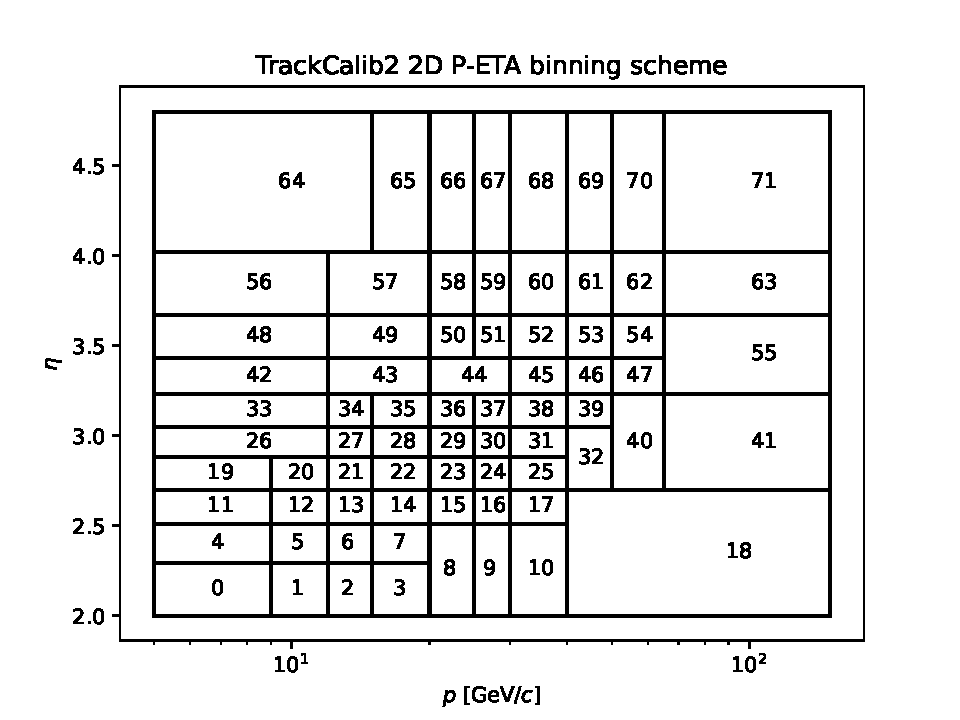
\includegraphics[width=0.8\textwidth]{Plots/TrackCalib2_2D_binning_scheme.pdf}
  \end{figure}
\end{frame}

\begin{frame}{2D binning}
  \vspace{0.0cm}
  \begin{figure}[htb]
    \centering
    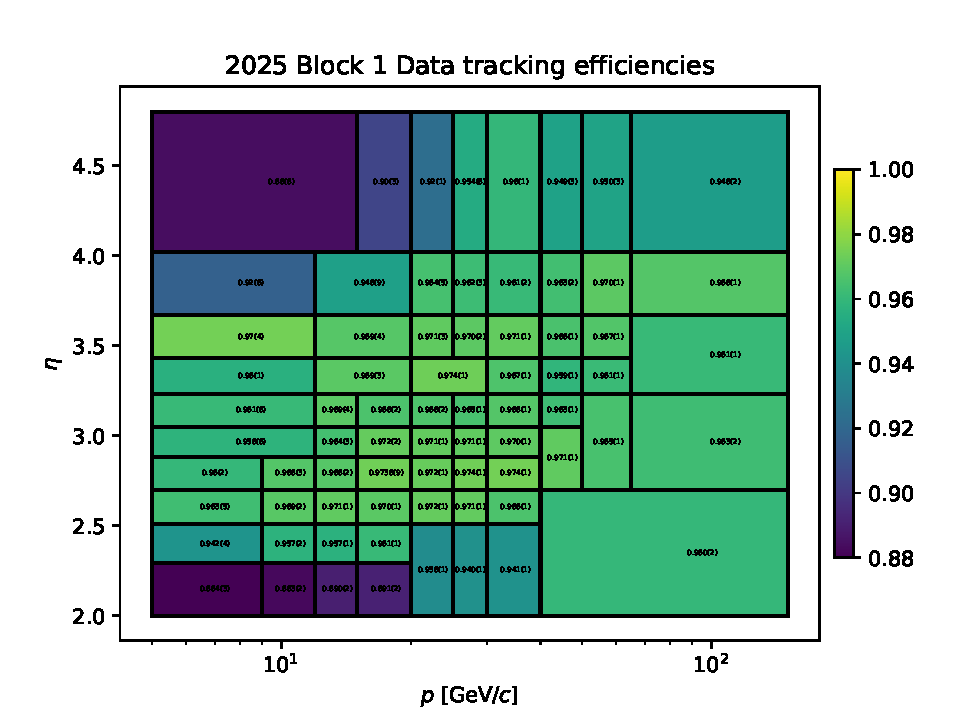
\includegraphics[width=0.85\textwidth]{Plots/TrackingEfficiencies_2D_binning_2025_Block1_Data_colour.pdf}
  \end{figure}
\end{frame}

\begin{frame}{2D binning}
  \vspace{0.0cm}
  \begin{figure}[htb]
    \centering
    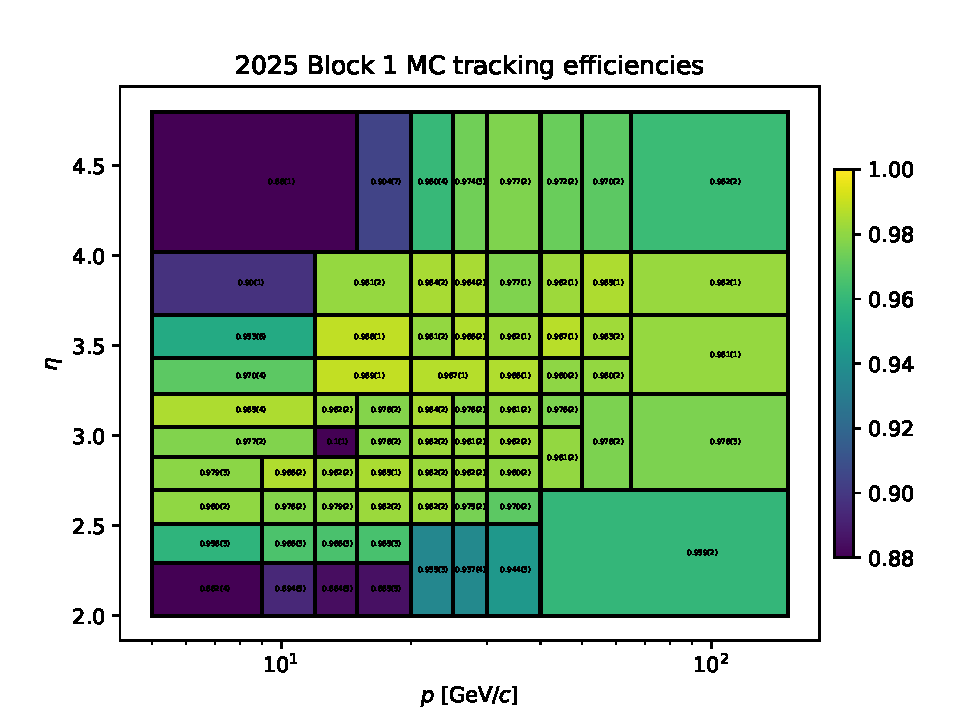
\includegraphics[width=0.85\textwidth]{Plots/TrackingEfficiencies_2D_binning_2025_Block1_MC_colour.pdf}
  \end{figure}
\end{frame}

\begin{frame}{2D binning}
  \vspace{0.0cm}
  \begin{figure}[htb]
    \centering
    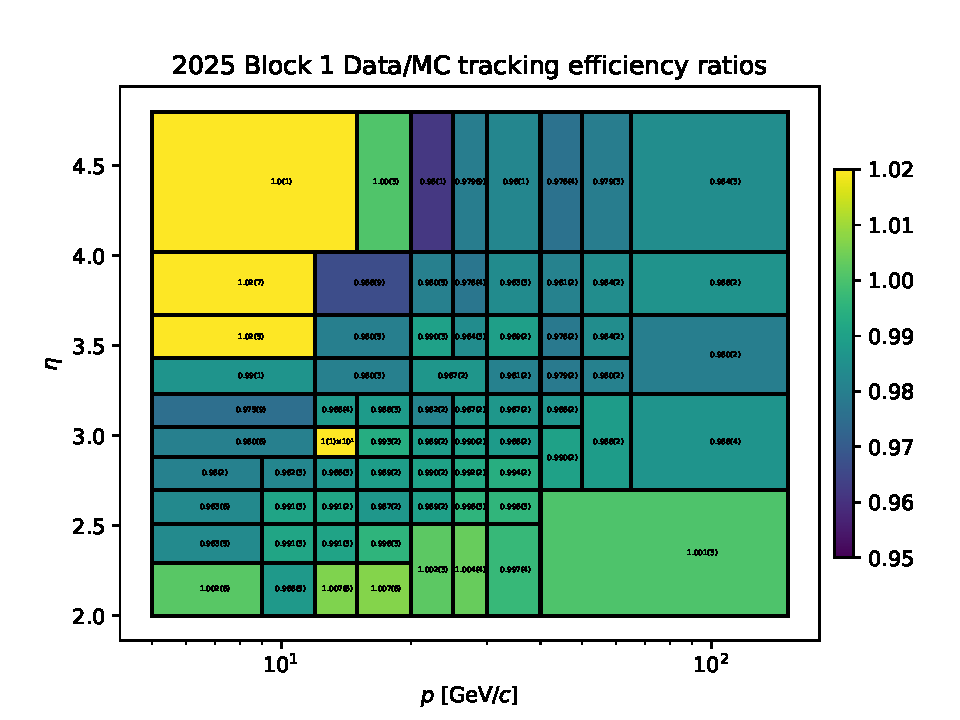
\includegraphics[width=0.85\textwidth]{Plots/TrackingEfficiencies_2D_binning_2025_Block1_Ratio_colour.pdf}
  \end{figure}
\end{frame}

\begin{frame}{2D binning}
  \vspace{0.0cm}
  \begin{figure}[htb]
    \centering
    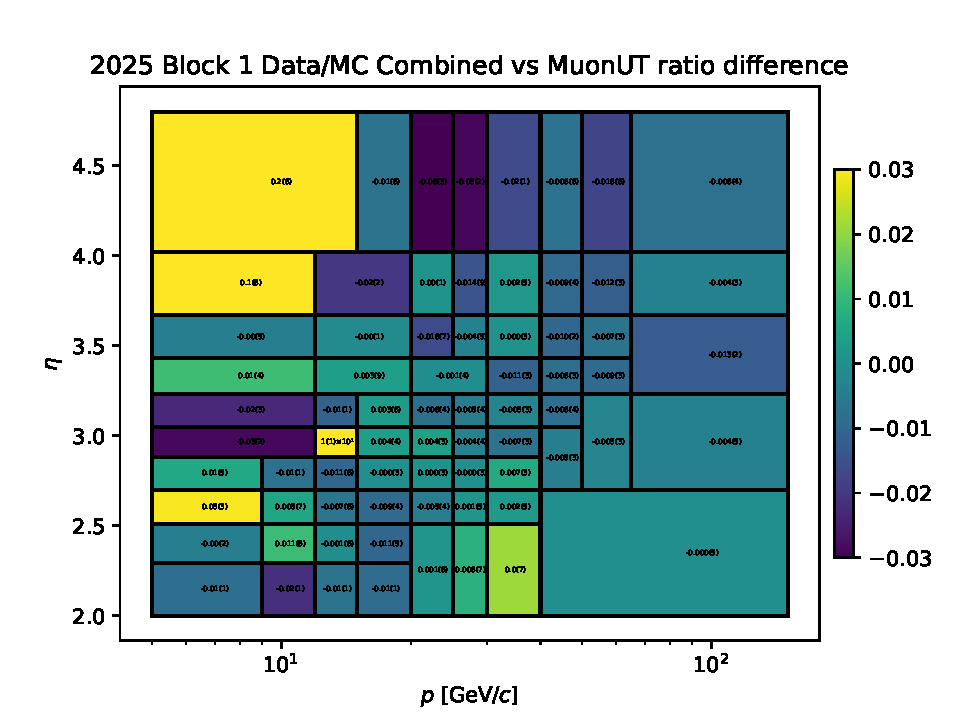
\includegraphics[width=0.85\textwidth]{Plots/TrackingEfficiencies_2D_binning_2025_Block1_RatioDiff_colour.pdf}
  \end{figure}
\end{frame}

\begin{frame}{2D binning}
  \vspace{0.0cm}
  \begin{figure}[htb]
    \centering
    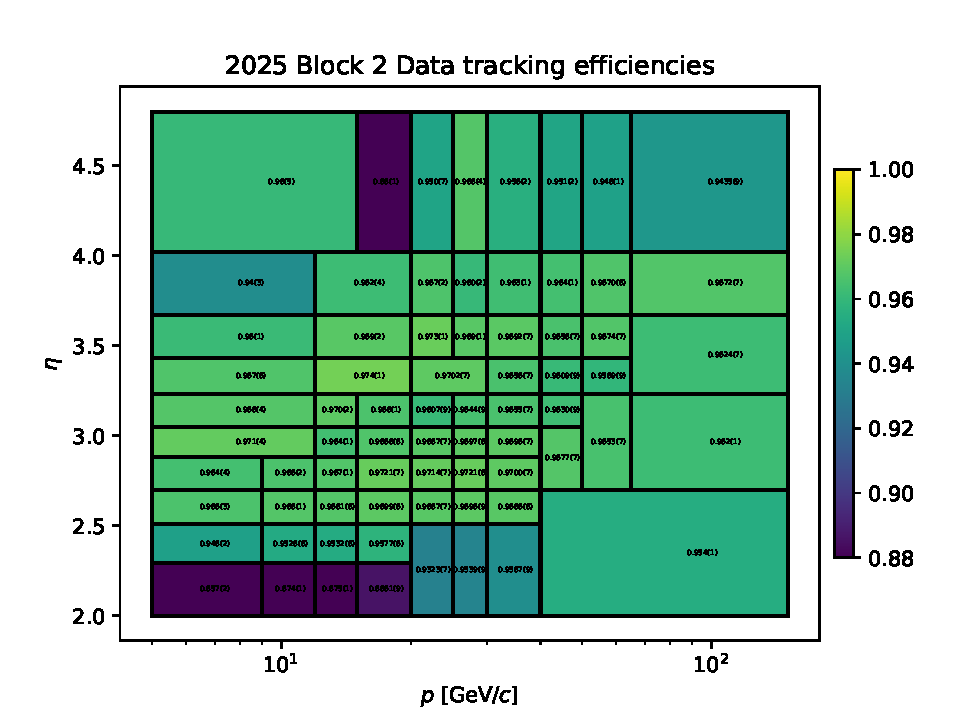
\includegraphics[width=0.85\textwidth]{Plots/TrackingEfficiencies_2D_binning_2025_Block2_Data_colour.pdf}
  \end{figure}
\end{frame}

\begin{frame}{2D binning}
  \vspace{0.0cm}
  \begin{figure}[htb]
    \centering
    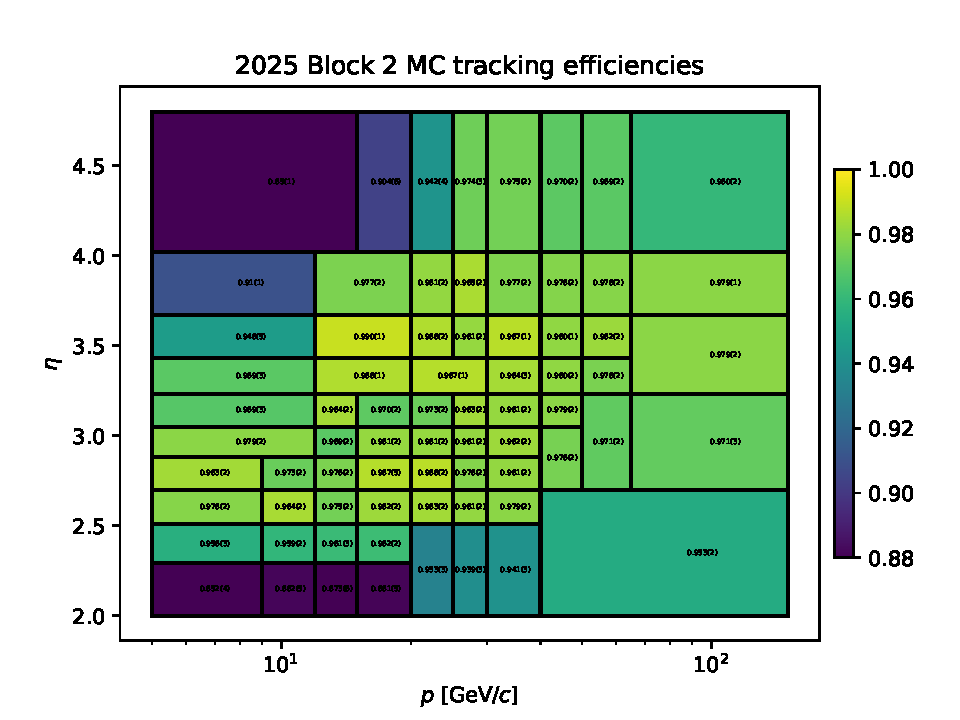
\includegraphics[width=0.85\textwidth]{Plots/TrackingEfficiencies_2D_binning_2025_Block2_MC_colour.pdf}
  \end{figure}
\end{frame}

\begin{frame}{2D binning}
  \vspace{0.0cm}
  \begin{figure}[htb]
    \centering
    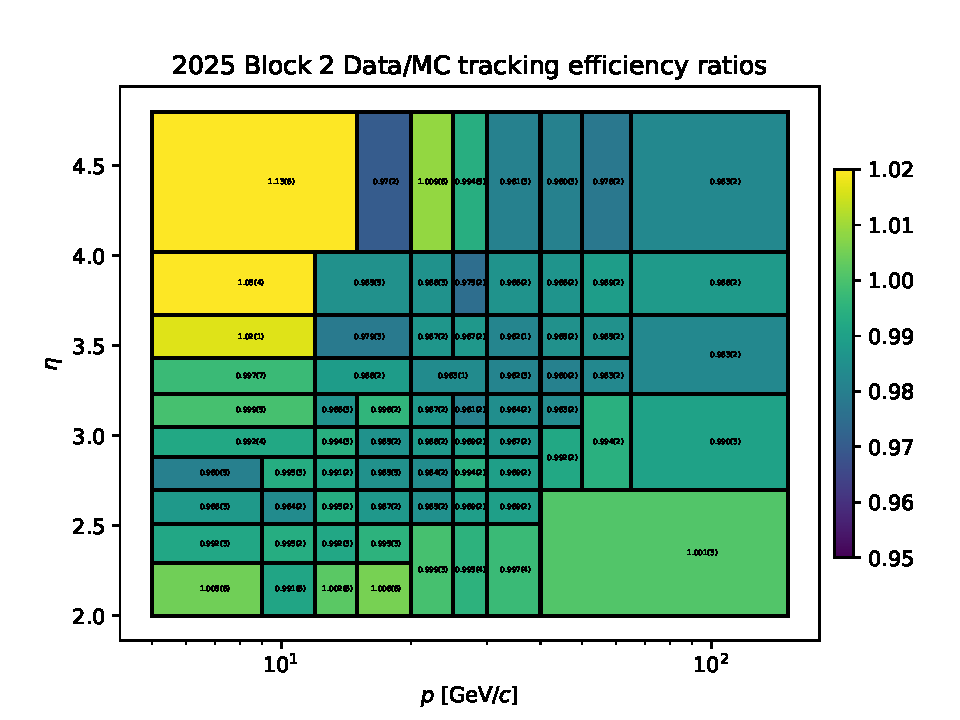
\includegraphics[width=0.85\textwidth]{Plots/TrackingEfficiencies_2D_binning_2025_Block2_Ratio_colour.pdf}
  \end{figure}
\end{frame}

\begin{frame}{2D binning}
  \vspace{0.0cm}
  \begin{figure}[htb]
    \centering
    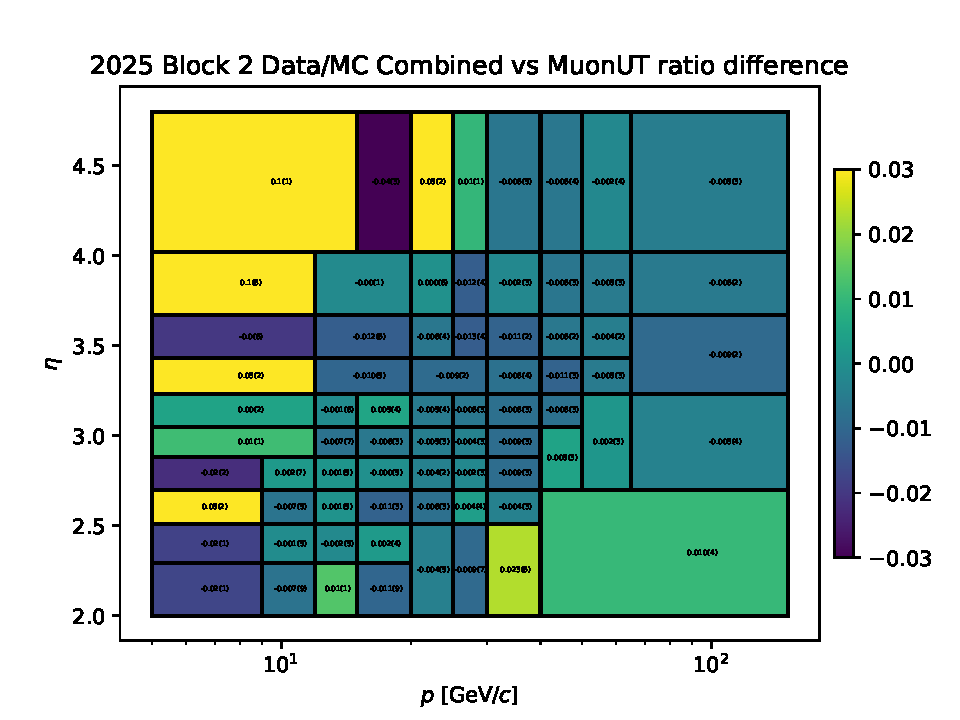
\includegraphics[width=0.85\textwidth]{Plots/TrackingEfficiencies_2D_binning_2025_Block2_RatioDiff_colour.pdf}
  \end{figure}
\end{frame}

\begin{frame}{Release of tracking efficiencies}
  \vspace{0.0cm}
  {\large We would like to release the tracking efficiency correction tables for 2025 pre-TS}
  \vspace{0.2cm}
  \begin{itemize}
    \setlength\itemsep{1.0em}
    \item{2024 v0 is already available on \href{https://gitlab.cern.ch/lhcb-rta/tracking-efficiencies-run-3}{GitLab}}
    \item{Add a file for 2025 with the same binning and same format}
    \item{Feedback is welcome!}
  \end{itemize}
\end{frame}

\begin{frame}{Initial look at 2026 efficiencies}
  \vspace{0.0cm}
  {\large Data SciFi efficiency comparison between 2025 and 2026}
  \begin{figure}[htb]
    \centering
    \begin{subfigure}{0.5\textwidth}
      \centering
      
\includegraphics[width=1.0\textwidth]{Plots/trackeff_Data_VeloMuon_P_workdir_samples.pdf}
    \end{subfigure}%
    \begin{subfigure}{0.5\textwidth}
      \centering
      
\includegraphics[width=1.0\textwidth]{Plots/trackeff_Data_VeloMuon_ETA_workdir_samples.pdf}
    \end{subfigure}
  \end{figure}
  \begin{itemize}
    \item{Drop in efficiencies over time, likely due to radiation damage}
    \item{Effect greater in region close to the beam (high $\eta$)}
  \end{itemize}
\end{frame}

\begin{frame}{Initial look at 2026 efficiencies}
  \vspace{0.0cm}
  {\large Data Velo efficiency comparison between 2025 and 2026}
  \begin{figure}[htb]
    \centering
    \begin{subfigure}{0.5\textwidth}
      \centering
      
\includegraphics[width=1.0\textwidth]{Plots/trackeff_Data_Downstream_P_workdir_samples.pdf}
    \end{subfigure}%
    \begin{subfigure}{0.5\textwidth}
      \centering
      
\includegraphics[width=1.0\textwidth]{Plots/trackeff_Data_Downstream_ETA_workdir_samples.pdf}
    \end{subfigure}
  \end{figure}
  \begin{itemize}
    \item{Clear drop in efficiencies in 2026 at high $p$ and in highest $\eta$ bin}
    \item{Most likely due to damage suffered during 2025 heavy ion run}
  \end{itemize}
\end{frame}

\begin{frame}{Summary and next steps}
  \vspace{0.0cm}
  {\large Summary:}
  \begin{enumerate}
    \item{Behaviour of 2025 tracking efficiencies understood}
    \item{Correction tables for pre-TS have been prepared}
    \item{Post-TS tables will follow once MC is ready}
    \item{See clear drop in Velo efficiencies in 2026 due to damage}
  \end{enumerate}
  \vspace{0.1cm}
  {\large Next steps}
  \begin{itemize}
    \item{Release 2025 post-TS tables (and 2026) once MC is available}
    \item{Finalise hadronic corrections}
    \item{Update tables using larger MC samples}
    \begin{itemize}
      \item{Revised P-ETA binning}
      \item{Separate tables for $\mu^+$ and $\mu^-$}
      \item{Charge integrated table with left and right bins in $\phi$}
    \end{itemize}
  \end{itemize}
  \vspace{0.0cm}
  \begin{center}
    \Huge Thanks for your attention!
  \end{center}
\end{frame}

\end{document}
